% Options for packages loaded elsewhere
\PassOptionsToPackage{unicode}{hyperref}
\PassOptionsToPackage{hyphens}{url}
%
\documentclass[
]{article}
\usepackage{amsmath,amssymb}
\usepackage{iftex}
\ifPDFTeX
  \usepackage[T1]{fontenc}
  \usepackage[utf8]{inputenc}
  \usepackage{textcomp} % provide euro and other symbols
\else % if luatex or xetex
  \usepackage{unicode-math} % this also loads fontspec
  \defaultfontfeatures{Scale=MatchLowercase}
  \defaultfontfeatures[\rmfamily]{Ligatures=TeX,Scale=1}
\fi
\usepackage{lmodern}
\ifPDFTeX\else
  % xetex/luatex font selection
\fi
% Use upquote if available, for straight quotes in verbatim environments
\IfFileExists{upquote.sty}{\usepackage{upquote}}{}
\IfFileExists{microtype.sty}{% use microtype if available
  \usepackage[]{microtype}
  \UseMicrotypeSet[protrusion]{basicmath} % disable protrusion for tt fonts
}{}
\makeatletter
\@ifundefined{KOMAClassName}{% if non-KOMA class
  \IfFileExists{parskip.sty}{%
    \usepackage{parskip}
  }{% else
    \setlength{\parindent}{0pt}
    \setlength{\parskip}{6pt plus 2pt minus 1pt}}
}{% if KOMA class
  \KOMAoptions{parskip=half}}
\makeatother
\usepackage{xcolor}
\usepackage[margin=1in]{geometry}
\usepackage{color}
\usepackage{fancyvrb}
\newcommand{\VerbBar}{|}
\newcommand{\VERB}{\Verb[commandchars=\\\{\}]}
\DefineVerbatimEnvironment{Highlighting}{Verbatim}{commandchars=\\\{\}}
% Add ',fontsize=\small' for more characters per line
\usepackage{framed}
\definecolor{shadecolor}{RGB}{248,248,248}
\newenvironment{Shaded}{\begin{snugshade}}{\end{snugshade}}
\newcommand{\AlertTok}[1]{\textcolor[rgb]{0.94,0.16,0.16}{#1}}
\newcommand{\AnnotationTok}[1]{\textcolor[rgb]{0.56,0.35,0.01}{\textbf{\textit{#1}}}}
\newcommand{\AttributeTok}[1]{\textcolor[rgb]{0.13,0.29,0.53}{#1}}
\newcommand{\BaseNTok}[1]{\textcolor[rgb]{0.00,0.00,0.81}{#1}}
\newcommand{\BuiltInTok}[1]{#1}
\newcommand{\CharTok}[1]{\textcolor[rgb]{0.31,0.60,0.02}{#1}}
\newcommand{\CommentTok}[1]{\textcolor[rgb]{0.56,0.35,0.01}{\textit{#1}}}
\newcommand{\CommentVarTok}[1]{\textcolor[rgb]{0.56,0.35,0.01}{\textbf{\textit{#1}}}}
\newcommand{\ConstantTok}[1]{\textcolor[rgb]{0.56,0.35,0.01}{#1}}
\newcommand{\ControlFlowTok}[1]{\textcolor[rgb]{0.13,0.29,0.53}{\textbf{#1}}}
\newcommand{\DataTypeTok}[1]{\textcolor[rgb]{0.13,0.29,0.53}{#1}}
\newcommand{\DecValTok}[1]{\textcolor[rgb]{0.00,0.00,0.81}{#1}}
\newcommand{\DocumentationTok}[1]{\textcolor[rgb]{0.56,0.35,0.01}{\textbf{\textit{#1}}}}
\newcommand{\ErrorTok}[1]{\textcolor[rgb]{0.64,0.00,0.00}{\textbf{#1}}}
\newcommand{\ExtensionTok}[1]{#1}
\newcommand{\FloatTok}[1]{\textcolor[rgb]{0.00,0.00,0.81}{#1}}
\newcommand{\FunctionTok}[1]{\textcolor[rgb]{0.13,0.29,0.53}{\textbf{#1}}}
\newcommand{\ImportTok}[1]{#1}
\newcommand{\InformationTok}[1]{\textcolor[rgb]{0.56,0.35,0.01}{\textbf{\textit{#1}}}}
\newcommand{\KeywordTok}[1]{\textcolor[rgb]{0.13,0.29,0.53}{\textbf{#1}}}
\newcommand{\NormalTok}[1]{#1}
\newcommand{\OperatorTok}[1]{\textcolor[rgb]{0.81,0.36,0.00}{\textbf{#1}}}
\newcommand{\OtherTok}[1]{\textcolor[rgb]{0.56,0.35,0.01}{#1}}
\newcommand{\PreprocessorTok}[1]{\textcolor[rgb]{0.56,0.35,0.01}{\textit{#1}}}
\newcommand{\RegionMarkerTok}[1]{#1}
\newcommand{\SpecialCharTok}[1]{\textcolor[rgb]{0.81,0.36,0.00}{\textbf{#1}}}
\newcommand{\SpecialStringTok}[1]{\textcolor[rgb]{0.31,0.60,0.02}{#1}}
\newcommand{\StringTok}[1]{\textcolor[rgb]{0.31,0.60,0.02}{#1}}
\newcommand{\VariableTok}[1]{\textcolor[rgb]{0.00,0.00,0.00}{#1}}
\newcommand{\VerbatimStringTok}[1]{\textcolor[rgb]{0.31,0.60,0.02}{#1}}
\newcommand{\WarningTok}[1]{\textcolor[rgb]{0.56,0.35,0.01}{\textbf{\textit{#1}}}}
\usepackage{graphicx}
\makeatletter
\newsavebox\pandoc@box
\newcommand*\pandocbounded[1]{% scales image to fit in text height/width
  \sbox\pandoc@box{#1}%
  \Gscale@div\@tempa{\textheight}{\dimexpr\ht\pandoc@box+\dp\pandoc@box\relax}%
  \Gscale@div\@tempb{\linewidth}{\wd\pandoc@box}%
  \ifdim\@tempb\p@<\@tempa\p@\let\@tempa\@tempb\fi% select the smaller of both
  \ifdim\@tempa\p@<\p@\scalebox{\@tempa}{\usebox\pandoc@box}%
  \else\usebox{\pandoc@box}%
  \fi%
}
% Set default figure placement to htbp
\def\fps@figure{htbp}
\makeatother
\setlength{\emergencystretch}{3em} % prevent overfull lines
\providecommand{\tightlist}{%
  \setlength{\itemsep}{0pt}\setlength{\parskip}{0pt}}
\setcounter{secnumdepth}{5}
\usepackage{booktabs}
\usepackage{longtable}
\usepackage{array}
\usepackage{multirow}
\usepackage{wrapfig}
\usepackage{float}
\usepackage{colortbl}
\usepackage{pdflscape}
\usepackage{tabu}
\usepackage{threeparttable}
\usepackage{threeparttablex}
\usepackage[normalem]{ulem}
\usepackage{makecell}
\usepackage{xcolor}
\usepackage{bookmark}
\IfFileExists{xurl.sty}{\usepackage{xurl}}{} % add URL line breaks if available
\urlstyle{same}
\hypersetup{
  pdftitle={Predicting the invasive species `Gorse (Ulex europaeus)' on the Banks Peninsula in New Zealand},
  hidelinks,
  pdfcreator={LaTeX via pandoc}}

\title{Predicting the invasive species `Gorse (Ulex europaeus)' on the
Banks Peninsula in New Zealand}
\usepackage{etoolbox}
\makeatletter
\providecommand{\subtitle}[1]{% add subtitle to \maketitle
  \apptocmd{\@title}{\par {\large #1 \par}}{}{}
}
\makeatother
\subtitle{Land cover classification with ML models in R}
\author{}
\date{\vspace{-2.5em}31 July, 2025}

\begin{document}
\maketitle

{
\setcounter{tocdepth}{6}
\tableofcontents
}
\section{Table of Contents}\label{table-of-contents}

\hyperref[statements]{Statements}

\hyperref[executive-summary]{Executive Summary}

\begin{enumerate}
\def\labelenumi{\arabic{enumi}.}
\item
  \hyperref[introduction]{Introduction}
\item
  \hyperref[aim-and-methodology-of-this-project]{Aim and Methodology of
  this Project}
\item
  \hyperref[exploratory-data-analysis-EDA]{Exploratory Data Analysis -
  EDA}

  \begin{itemize}
  \item
    \hyperref[data-loading]{Data Loading}
  \item
    \hyperref[data-pre-processing]{Data Pre-processing}
  \end{itemize}
\item
  \hyperref[machine-learning-model]{Machine Learning Model}

  \begin{itemize}
  \item
    \hyperref[random-forest]{Random Forest}
  \item
    \hyperref[xgboost]{XGBoost}
  \item
    \hyperref[support-vector-machine-svm]{Support Vector Machine (SVM)}
  \end{itemize}
\item
  \hyperref[results]{Results}

  \begin{itemize}
  \item
    \hyperref[predicted-maps]{Predicted Maps}
  \item
    \hyperref[model-performance-ux26-uncertainity-analysis]{Model
    Performance \& Uncertainity Analysis}
  \end{itemize}
\item
  \hyperref[conclusion]{Conclusion}
\end{enumerate}

\section{Statements}\label{statements}

\textbf{Acknowledgement} I am sincerely thank the OpenGeoHub Foundation
for their work in making open source geospatial models for everyone. The
videos posted in their website on tutorials to learn remote sensing
concepts and understand the workflow structures in working with
geospatial data analysis. Particular mention to the tutorial
\emph{``Machine Learning for Spatial Data''} by Dr.~Hanna Meyer which
helped me to work on this project.

Furthermore, I thank the professional czertification courses relevant to
understanding programming, machine learning, remote sensing concepts
which helped me to work on this project.

\textbf{Use of generative artificial intelligence} Generative artificial
intelligence (GenAI) was mainly used for creating charts and adjusting
visualization parameters in R. GenAI was also used for code debugging.
However, the responses provided by GenAI were critically judged before
being implemented.

\section{Executive Summary}\label{executive-summary}

\textbf{Problem Statement} \textbf{Gorse (\emph{Ulex europaeus})} plant
was brought to New Zealand during the European settlement as a hedge
plant and spreads into farmlands which is associated with negative
consequences for the quality of the grassland. Each year millions of
dollars are spent for its control and field sampling are expensive for
developing management strategies. It's of high importance to map the
distribution of such invasive plants using remote sensing methods.

\textbf{Project Aim and Focus} The project aim and focus is on using
Machine Learning models to predict the invasive species \textbf{gorse
(\emph{Ulex europaeus})} on the Banks Peninsula of New Zealand.

\textbf{Raw data used} Sentinel satellite data and plotted land cover
class of a section of the Banks Peninsula of New Zealand.

\textbf{Methodology} The following methodology was undertaken for this
project,

\begin{itemize}
\item
  Raw data and land cover classes are visualized and merged to a single
  data set to build the Machine Learning models
  (\texttt{Random\ Forest}, \texttt{XGBoost} and
  \texttt{Support\ Vector\ Machine}).
\item
  The merged data set is split into 30\% training and 70\% test data
  which is used to train and predict using the models.
\item
  Various analysis such as confusion matrix, scoring metrics, predictive
  \& entropy maps, and uncertainty diagnostics were performed to analyse
  the models performance in land cover classification and predicting the
  invasive plant species.
\end{itemize}

\textbf{Results} Out of the three models, \texttt{RF} and
\texttt{XGBoost} model performs very well and \texttt{SVM} model is not
up to par in classifying the land cover class using the satellite
images. Based on the various analysis, \texttt{Random\ Forest} with the
highest accuracy of 99.33\%, Model outperforms \texttt{XGBoost} in
predicting the invasive species \textbf{gorse (\emph{Ulex europaeus})},
using Sentinel satellite data, on the Banks Peninsula of NewZealand.

\section{1. Introduction}\label{introduction}

This project demonstrates land cover classifications in R using machine
learning algorithms such as \texttt{Random\ Forest}, \texttt{XGBoost},
and \texttt{SVM}, and compares their performance. This was adapted from
the tutorial presented by Dr.~Hanna Meyer in July 2018 and has been
adapted to include additional machine learning models for comparison.

The focus is on land cover classification using sentinel satellite data,
specifically targeting the invasive species \textbf{gorse (\emph{Ulex
europaeus})} on the Banks Peninsula. This plant was brought to New
Zealand during the European settlement as a hedge plant and spreads into
farmland which is associated with negative consequences for the quality
of the grassland.

Each year millions of dollars are spent for its control. To develop
management strategies, it's of high importance to map the distribution
of such invasive plants. Since field sampling means huge expenses,
remote sensing methods are required for a spatially explicit monitoring.
In this tutorial, we're going to use Sentinel satellite imagery from
2017 to map the current land cover distribution on a section of the
Banks Peninsula.

\section{\texorpdfstring{2. Aim and \textbf{Methodology} of this
Project}{2. Aim and Methodology of this Project}}\label{aim-of-this-project}

The project aim is to predict the invasive species \textbf{gorse
(\emph{Ulex europaeus})} on the Banks Peninsula and focus on using
machine learning algorithms such as Random Forests, XGBoost and SVM to
perform this project. We show its performance and compare the results of
the models.

The following methodology was undertaken for this project,

\begin{itemize}
\item
  Raw data and land cover classes are visualized and merged to a single
  data set to build the Machine Learning models
  (\texttt{Random\ Forest}, \texttt{XGBoost} and
  \texttt{Support\ Vector\ Machine}).
\item
  The merged data set is split into 30\% training and 70\% test data
  which is used to train and predict using the models.
\item
  Various analysis such as confusion matrix, scoring metrics, predictive
  \& entropy maps, and uncertainty diagnostics were performed to analyse
  the models performance in land cover classification and predicting the
  invasive plant species.
\end{itemize}

\section{3. Exploratory Data Analysis -
EDA}\label{exploratory-data-analysis---eda}

This project shows the process of land cover (LC) classification using
machine learning techniques using R. The focus is on classifying land
cover types, particularly the invasive species \textbf{gorse (\emph{Ulex
europaeus})}, using Sentinel satellite data.

\subsection{Load required libraries}\label{load-required-libraries}

First, loading the libraries and packages that are needed for this LC
classification project. The selected libraries provide functions for
handling raster data, reading shapefiles, performing machine learning
tasks, and visualizing results.

\begin{Shaded}
\begin{Highlighting}[]
\NormalTok{knitr}\SpecialCharTok{::}\NormalTok{opts\_chunk}\SpecialCharTok{$}\FunctionTok{set}\NormalTok{(}\AttributeTok{echo =} \ConstantTok{TRUE}\NormalTok{)}

\CommentTok{\# Spatial and Raster data handling packages}
\FunctionTok{library}\NormalTok{(raster)       }\CommentTok{\# Handling Raster data }
\FunctionTok{library}\NormalTok{(sf)           }\CommentTok{\# Handling Vector data }
\FunctionTok{library}\NormalTok{(terra)        }\CommentTok{\# Optimise large raster datasets }
\FunctionTok{library}\NormalTok{(mapview)      }\CommentTok{\# Quick raster/vector visualization}

\CommentTok{\# Data Manipulation \& Reshaping}
\FunctionTok{library}\NormalTok{(dplyr)        }\CommentTok{\# Data wrangling }
\FunctionTok{library}\NormalTok{(tidyr)        }\CommentTok{\# Data reshaping}
\FunctionTok{library}\NormalTok{(reshape2)     }\CommentTok{\# Data reshaping (melt/cast)}
\FunctionTok{library}\NormalTok{(ROSE)         }\CommentTok{\# Balancing imbalanced datasets }

\CommentTok{\# Model Building \& Machine Learning packages}
\FunctionTok{library}\NormalTok{(caret)        }\CommentTok{\# Model building}
\FunctionTok{library}\NormalTok{(randomForest) }\CommentTok{\# Random Forest}
\FunctionTok{library}\NormalTok{(xgboost)      }\CommentTok{\# XGBoost}
\FunctionTok{library}\NormalTok{(e1071)        }\CommentTok{\# SVM }
\FunctionTok{library}\NormalTok{(rpart)        }\CommentTok{\# Recursive partitioning and Regression Trees}
\FunctionTok{library}\NormalTok{(ranger)       }\CommentTok{\# Faster implementaion of RF }

\CommentTok{\# Model Evaluation and Interpretation packages}
\FunctionTok{library}\NormalTok{(ModelMetrics) }\CommentTok{\# Performance Metrics }
\FunctionTok{library}\NormalTok{(pROC)         }\CommentTok{\# ROC and AUC curves }
\FunctionTok{library}\NormalTok{(DALEX)        }\CommentTok{\# Model explainability: }
\FunctionTok{library}\NormalTok{(ingredients)  }\CommentTok{\# Aligns with DALEX}
\FunctionTok{library}\NormalTok{(vip)          }\CommentTok{\# Visualizing feature importance }


\CommentTok{\# Visualization, Plotting \& Reporting packages}
\FunctionTok{library}\NormalTok{(ggplot2)      }\CommentTok{\# Powerful and flexible plotting }
\FunctionTok{library}\NormalTok{(RColorBrewer) }\CommentTok{\# Predefined color palettes}
\FunctionTok{library}\NormalTok{(rasterVis)    }\CommentTok{\# Customized raster visualization}
\FunctionTok{library}\NormalTok{(kableExtra)   }\CommentTok{\# Table styling}
\FunctionTok{library}\NormalTok{(viridis)      }\CommentTok{\# Colorblind{-}friendly maps}
\FunctionTok{library}\NormalTok{(tinytex)      }\CommentTok{\# Compile LaTeX docs}
\end{Highlighting}
\end{Shaded}

\subsection{Data Loading and
Pre-processing}\label{data-loading-and-pre-processing}

\subsubsection{Load and explore the
data}\label{load-and-explore-the-data}

To start with, loading the Sentinel data as well as a land cover class
of the training sites.

\begin{Shaded}
\begin{Highlighting}[]
\CommentTok{\# Load Sentinel data}
\NormalTok{sentinel }\OtherTok{\textless{}{-}} \FunctionTok{stack}\NormalTok{(}\StringTok{"D:}\SpecialCharTok{\textbackslash{}\textbackslash{}}\StringTok{Study}\SpecialCharTok{\textbackslash{}\textbackslash{}}\StringTok{Machine Learning}\SpecialCharTok{\textbackslash{}\textbackslash{}}\StringTok{Geostatistics}\SpecialCharTok{\textbackslash{}\textbackslash{}}\StringTok{R{-}Git}\SpecialCharTok{\textbackslash{}\textbackslash{}}\StringTok{Case{-}Study\_ML{-}for{-}Spatial{-}Data}\SpecialCharTok{\textbackslash{}\textbackslash{}}\StringTok{Data}\SpecialCharTok{\textbackslash{}\textbackslash{}}\StringTok{sentinel2017.grd"}\NormalTok{)}

\CommentTok{\# Load training sites shapefile}
\NormalTok{training }\OtherTok{\textless{}{-}} \FunctionTok{read\_sf}\NormalTok{(}\StringTok{"D:}\SpecialCharTok{\textbackslash{}\textbackslash{}}\StringTok{Study}\SpecialCharTok{\textbackslash{}\textbackslash{}}\StringTok{Machine Learning}\SpecialCharTok{\textbackslash{}\textbackslash{}}\StringTok{Geostatistics}\SpecialCharTok{\textbackslash{}\textbackslash{}}\StringTok{R{-}Git}\SpecialCharTok{\textbackslash{}\textbackslash{}}\StringTok{Case{-}Study\_ML{-}for{-}Spatial{-}Data}\SpecialCharTok{\textbackslash{}\textbackslash{}}\StringTok{Data}\SpecialCharTok{\textbackslash{}\textbackslash{}}\StringTok{trainingSites.shp"}\NormalTok{)}

\CommentTok{\# Visualize the Sentinel data}
\FunctionTok{print}\NormalTok{(sentinel)}
\end{Highlighting}
\end{Shaded}

\begin{verbatim}
## class      : RasterStack 
## dimensions : 1257, 1405, 1766085, 10  (nrow, ncol, ncell, nlayers)
## resolution : 10, 10  (x, y)
## extent     : 655950, 670000, 5138290, 5150860  (xmin, xmax, ymin, ymax)
## crs        : +proj=utm +zone=59 +south +ellps=WGS84 +towgs84=0,0,0,0,0,0,0 +units=m +no_defs 
## names      :          B02,          B03,          B04,          B08,          B05,          B06,          B07,          B8A,         NDVI,   yellowness 
## min values :  619.0000000,  373.0000000,  194.0000000,   98.0000000,  168.3125000,  155.1875000,  139.0625000,  100.1875000,   -0.6810878,   -0.1066810 
## max values : 5385.0000000, 5137.0000000, 5289.0000000, 6984.0000000, 4209.0625000, 5333.6875000, 6705.6875000, 7297.2500000,    0.8989085,    0.5362146
\end{verbatim}

\begin{Shaded}
\begin{Highlighting}[]
\FunctionTok{print}\NormalTok{(training)}
\end{Highlighting}
\end{Shaded}

\begin{verbatim}
## Simple feature collection with 23 features and 2 fields
## Geometry type: POLYGON
## Dimension:     XY
## Bounding box:  xmin: 656358 ymin: 5138445 xmax: 669091.9 ymax: 5150851
## Projected CRS: WGS 84 / UTM zone 59S
## # A tibble: 23 x 3
##       id Class                                                          geometry
##    <dbl> <chr>                                                     <POLYGON [m]>
##  1     1 Gorse     ((660956.4 5146064, 661018.8 5146061, 661033.1 5146008, 6609~
##  2     2 Gorse     ((661120.6 5146267, 661197.3 5146263, 661205.7 5146231, 6611~
##  3     3 Gorse     ((662279.2 5148528, 662388.2 5148465, 662382.2 5148421, 6622~
##  4     4 Gorse     ((663908.7 5148424, 664023.7 5148401, 664054.9 5148404, 6641~
##  5     5 Gorse     ((662357.1 5145141, 662514 5145113, 662547.6 5145081, 662636~
##  6     6 Water     ((668392.1 5144225, 669091.9 5143123, 668248.4 5143200, 6683~
##  7     7 Water     ((665171.5 5138877, 666369.7 5138445, 665401.6 5138522, 6651~
##  8     8 Water     ((656358 5147753, 656722.2 5147403, 656444.2 5147446, 656358~
##  9     9 Grassland ((658817.8 5146617, 658875.3 5146725, 658936.4 5146717, 6589~
## 10    10 Grassland ((659407.2 5140035, 659565.4 5139956, 659539 5139786, 659457~
## # i 13 more rows
\end{verbatim}

\textbf{Overview of the data:} The Sentinel data is a stack of raster
layers, The sentinel data subset for this tutorial contains the Sentinel
channels 2-8 (visible and near infrared channels) as well as the NDVI
and a yellowness index that was calculated as
(red+green-blue)/(red+green+blue) as additional bands. We assume the
yellowness index is valuable to distinguish the striking yellow color of
the gorse from other vegetation.To get an idea about the band
composition and spatial resolution, please check the Sentinel Wikipedia
documentation
\href{https://en.wikipedia.org/wiki/Sentinel-2\#Data_products}{here}.
The training sites are polygons that were digitized in QGIS on the basis
of the Sentinel data using expert knowledge. The training dataset
contains different land cover types, including gorse, grassland, and
other vegetation types.

\textbf{Visualize the data:} We visualize the Sentinel data as a true
color composite in the geographical context and overlay it with the
polygons. Click on the polygons to see which land cover class is
assigned to a respective polygon.

\begin{Shaded}
\begin{Highlighting}[]
\CommentTok{\# Visualize Sentinel data with training sites}
\FunctionTok{viewRGB}\NormalTok{(sentinel, }\AttributeTok{r=}\DecValTok{3}\NormalTok{, }\AttributeTok{g=}\DecValTok{2}\NormalTok{, }\AttributeTok{b=}\DecValTok{1}\NormalTok{, }\AttributeTok{map.types =} \StringTok{"Esri.WorldImagery"}\NormalTok{) }\SpecialCharTok{+} 
  \FunctionTok{mapview}\NormalTok{(training)}
\end{Highlighting}
\end{Shaded}

\subsubsection{Data Pre-processing}\label{data-pre-processing}

We need to prepare the data for machine learning by extracting raster
values for the training sites and merging them with the land cover class
information from the training shape file. This step is crucial for
training the machine learning model. Then, we split the data into
training and test data set to ensure that we can evaluate the model's
performance on unseen data.

\textbf{Extract raster information:} In order to train the Machine
Learning model between the spectral properties and the land cover class,
we first need to create a data frame that contains the spectral
properties of the training sites as well as the corresponding class
information. This data frame can be produced with the \texttt{extract}
function. The resulting data frame contains the Sentinel data for each
pixel overlayed by the polygons. This data frame then still needs to be
merged with the information on the land cover class from the shape file.
This happens via the ID of the polygons which are given in the extracted
data frame by the column ``ID'' and in the shape file by the attribute
``id''.

\begin{Shaded}
\begin{Highlighting}[]
\CommentTok{\# Extract raster values for training sites}
\NormalTok{extr }\OtherTok{\textless{}{-}}\NormalTok{ raster}\SpecialCharTok{::}\FunctionTok{extract}\NormalTok{(sentinel, training, }\AttributeTok{df=}\ConstantTok{TRUE}\NormalTok{)}

\CommentTok{\# Merge extracted data with training sites}
\NormalTok{extr }\OtherTok{\textless{}{-}} \FunctionTok{merge}\NormalTok{(extr, training, }\AttributeTok{by.x=}\StringTok{"ID"}\NormalTok{, }\AttributeTok{by.y=}\StringTok{"id"}\NormalTok{)}
\FunctionTok{kable}\NormalTok{(}\FunctionTok{head}\NormalTok{(extr), }\AttributeTok{caption =} \StringTok{"Merged Data"}\NormalTok{) }\SpecialCharTok{\%\textgreater{}\%}
  \FunctionTok{kable\_styling}\NormalTok{(}\AttributeTok{full\_width =}\NormalTok{ F, }\AttributeTok{position =} \StringTok{"left"}\NormalTok{)}
\end{Highlighting}
\end{Shaded}

\begin{longtable}[l]{rrrrrrrrrrrll}
\caption{\label{tab:extract}Merged Data}\\
\toprule
ID & B02 & B03 & B04 & B08 & B05 & B06 & B07 & B8A & NDVI & yellowness & Class & geometry\\
\midrule
1 & 767 & 1113 & 1095 & 2854 & 1425.688 & 2358.625 & 2791.750 & 3091.375 & 0.4454292 & 0.4843698 & Gorse & POLYGON ((660956.4 5146064,...\\
1 & 767 & 1049 & 1029 & 2667 & 1409.000 & 2320.438 & 2742.688 & 3037.125 & 0.4431818 & 0.4608084 & Gorse & POLYGON ((660956.4 5146064,...\\
1 & 767 & 956 & 910 & 2444 & 1367.500 & 2213.312 & 2617.562 & 2923.375 & 0.4573644 & 0.4173946 & Gorse & POLYGON ((660956.4 5146064,...\\
1 & 760 & 944 & 918 & 2418 & 1347.500 & 2184.625 & 2574.375 & 2874.875 & 0.4496403 & 0.4202898 & Gorse & POLYGON ((660956.4 5146064,...\\
1 & 743 & 1017 & 981 & 2543 & 1349.000 & 2234.375 & 2613.125 & 2891.625 & 0.4432463 & 0.4578621 & Gorse & POLYGON ((660956.4 5146064,...\\
\addlinespace
1 & 737 & 991 & 939 & 2648 & 1352.000 & 2256.250 & 2637.562 & 2922.500 & 0.4764427 & 0.4473191 & Gorse & POLYGON ((660956.4 5146064,...\\
\bottomrule
\end{longtable}

\textbf{Splitting data into training and test data:} In order to keep
data for a later (nearly) independent validation as well as to limit the
number of data points so that the model training won't take long time,
splitting the total data set into 30\% training data and 70\% test data
is necessary. The more testing (unknown) data the higher the model
accuracy. Caret's \texttt{createDataPartition} takes care that the class
distribution is the same in both data sets.

\begin{Shaded}
\begin{Highlighting}[]
\CommentTok{\# Set seed for reproducibility}
\FunctionTok{set.seed}\NormalTok{(}\DecValTok{100}\NormalTok{)}

\CommentTok{\# Create training and test dataset}
\NormalTok{trainids }\OtherTok{\textless{}{-}} \FunctionTok{createDataPartition}\NormalTok{(extr}\SpecialCharTok{$}\NormalTok{Class, }\AttributeTok{list=}\ConstantTok{FALSE}\NormalTok{, }\AttributeTok{p=}\FloatTok{0.3}\NormalTok{)}
\NormalTok{trainDat }\OtherTok{\textless{}{-}}\NormalTok{ extr[trainids,]}
\NormalTok{testDat }\OtherTok{\textless{}{-}}\NormalTok{ extr[}\SpecialCharTok{{-}}\NormalTok{trainids,]}

\CommentTok{\# Ensure Class is a factor and is at the same level}
\NormalTok{trainDat}\SpecialCharTok{$}\NormalTok{Class }\OtherTok{\textless{}{-}} \FunctionTok{factor}\NormalTok{(trainDat}\SpecialCharTok{$}\NormalTok{Class)}
\NormalTok{testDat}\SpecialCharTok{$}\NormalTok{Class }\OtherTok{\textless{}{-}} \FunctionTok{factor}\NormalTok{(testDat}\SpecialCharTok{$}\NormalTok{Class)}

\CommentTok{\# Check the distribution of classes in training and test datasets}
\NormalTok{training\_class }\OtherTok{=} \FunctionTok{round}\NormalTok{(}\FunctionTok{prop.table}\NormalTok{(}\FunctionTok{table}\NormalTok{(trainDat}\SpecialCharTok{$}\NormalTok{Class)) }\SpecialCharTok{*} \DecValTok{100}\NormalTok{, }\DecValTok{2}\NormalTok{)}
\NormalTok{test\_class }\OtherTok{=} \FunctionTok{round}\NormalTok{(}\FunctionTok{prop.table}\NormalTok{(}\FunctionTok{table}\NormalTok{(testDat}\SpecialCharTok{$}\NormalTok{Class)) }\SpecialCharTok{*} \DecValTok{100}\NormalTok{, }\DecValTok{2}\NormalTok{)}

\FunctionTok{kable}\NormalTok{(training\_class, }\AttributeTok{caption =} \StringTok{"Training class balance"}\NormalTok{) }\SpecialCharTok{\%\textgreater{}\%}
  \FunctionTok{kable\_styling}\NormalTok{(}\AttributeTok{full\_width =}\NormalTok{ F, }\AttributeTok{position =} \StringTok{"left"}\NormalTok{)}
\end{Highlighting}
\end{Shaded}

\begin{longtable}[l]{lr}
\caption{\label{tab:split}Training class balance}\\
\toprule
Var1 & Freq\\
\midrule
Bare & 5.73\\
Bush & 9.21\\
Forestry & 9.27\\
Gorse & 7.96\\
Grassland & 6.41\\
\addlinespace
Sand & 2.81\\
Urban & 2.28\\
Water & 56.33\\
\bottomrule
\end{longtable}

\begin{Shaded}
\begin{Highlighting}[]
\FunctionTok{kable}\NormalTok{(test\_class, }\AttributeTok{caption =} \StringTok{"Test class balance"}\NormalTok{) }\SpecialCharTok{\%\textgreater{}\%}
  \FunctionTok{kable\_styling}\NormalTok{(}\AttributeTok{full\_width =}\NormalTok{ F, }\AttributeTok{position =} \StringTok{"left"}\NormalTok{)}
\end{Highlighting}
\end{Shaded}

\begin{longtable}[l]{lr}
\caption{\label{tab:split}Test class balance}\\
\toprule
Var1 & Freq\\
\midrule
Bare & 5.71\\
Bush & 9.20\\
Forestry & 9.27\\
Gorse & 7.96\\
Grassland & 6.39\\
\addlinespace
Sand & 2.77\\
Urban & 2.29\\
Water & 56.40\\
\bottomrule
\end{longtable}

Class balance inferences shows that there are severe class imbalance
within both training and test data sets. It is required to balance the
class using up-sampling as the \texttt{Water} has a high frequency and
the remaining classes are similar to each other and much lower that the
\texttt{Water}.

\textbf{Visualize relationships:} To get an idea about the relationships
between the spectral Sentinel data and the land cover class, we can
visualize how the different bands differs according to the land cover
class. This helps us understand the distribution of different classes in
the feature space.

\begin{Shaded}
\begin{Highlighting}[]
\CommentTok{\# Visualize relationships (box plot) between yellowness index and land cover class}
\FunctionTok{ggplot}\NormalTok{(trainDat, }\FunctionTok{aes}\NormalTok{(}\AttributeTok{x =} \FunctionTok{factor}\NormalTok{(Class), }\AttributeTok{y =}\NormalTok{ yellowness)) }\SpecialCharTok{+}
  \FunctionTok{geom\_boxplot}\NormalTok{() }\SpecialCharTok{+}
  \FunctionTok{labs}\NormalTok{(}\AttributeTok{title =} \StringTok{"Yellowness Index by Land Cover Class"}\NormalTok{,}
       \AttributeTok{x =} \StringTok{"Land Cover Class"}\NormalTok{,}
       \AttributeTok{y =} \StringTok{"Yellowness Index"}\NormalTok{) }\SpecialCharTok{+}
  \FunctionTok{theme\_minimal}\NormalTok{()}
\end{Highlighting}
\end{Shaded}

\pandocbounded{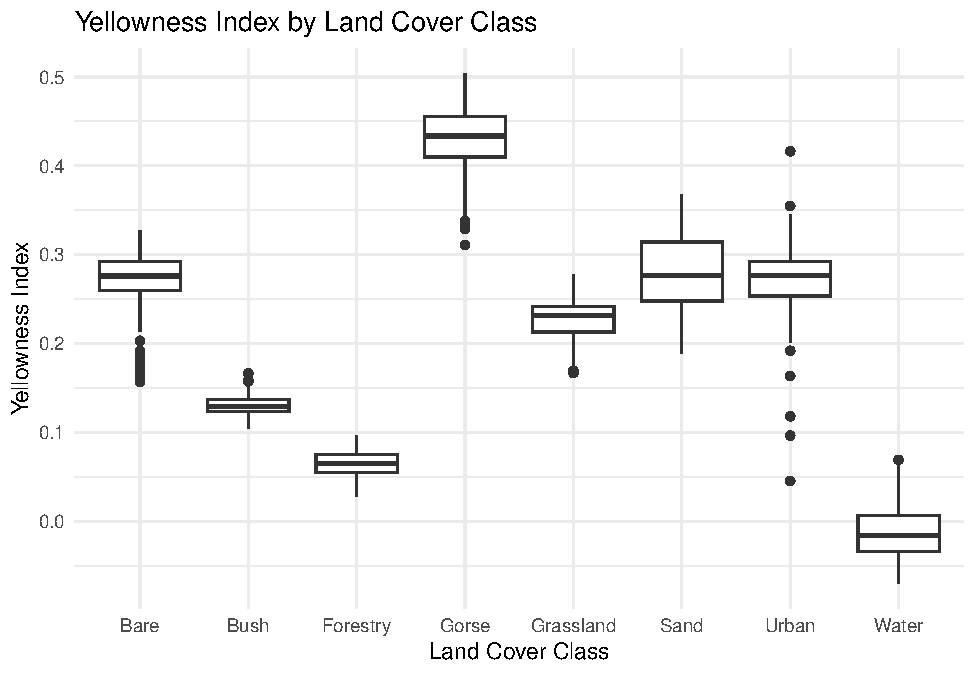
\includegraphics[keepaspectratio]{ML-based-modelling-for-spatial-and-spatiotemporal-data_files/figure-latex/vis_relationships-1.pdf}}

\begin{Shaded}
\begin{Highlighting}[]
\CommentTok{\# Visualize relationships (box plot) between NDVI and land cover class}
\FunctionTok{ggplot}\NormalTok{(trainDat, }\FunctionTok{aes}\NormalTok{(}\AttributeTok{x =} \FunctionTok{factor}\NormalTok{(Class), }\AttributeTok{y =}\NormalTok{ NDVI)) }\SpecialCharTok{+}
  \FunctionTok{geom\_boxplot}\NormalTok{() }\SpecialCharTok{+}
  \FunctionTok{labs}\NormalTok{(}\AttributeTok{title =} \StringTok{"NDVI by Land Cover Class"}\NormalTok{,}
       \AttributeTok{x =} \StringTok{"Land Cover Class"}\NormalTok{,}
       \AttributeTok{y =} \StringTok{"NDVI"}\NormalTok{) }\SpecialCharTok{+}
  \FunctionTok{theme\_minimal}\NormalTok{()}
\end{Highlighting}
\end{Shaded}

\pandocbounded{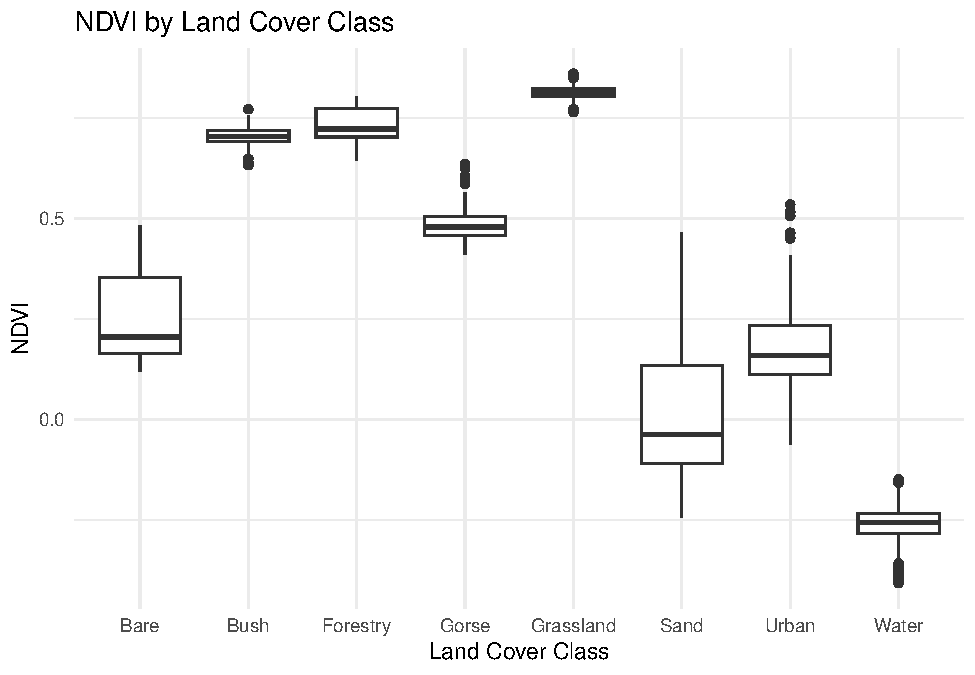
\includegraphics[keepaspectratio]{ML-based-modelling-for-spatial-and-spatiotemporal-data_files/figure-latex/vis_relationships-2.pdf}}

The box plots show the distribution of the yellowness index and NDVI for
each land cover class, providing insights into how these indices vary
across different classes. The Gorse class features the highest
``yellowness'' values while all other land cover classes have
considerably lower values.

\textbf{Feature Plot:} We can also get an impression about the
separability of the classes by creating a feature plot that visualizes
the location of the training samples in a scatter plot of two Sentinel
channels.

\begin{Shaded}
\begin{Highlighting}[]
\CommentTok{\# Create feature plot to visualize relationships between Sentinel channels (B08 vs yellowness) and land cover class}
\FunctionTok{ggplot}\NormalTok{(trainDat, }\FunctionTok{aes}\NormalTok{(}\AttributeTok{x =}\NormalTok{ B08, }\AttributeTok{y =}\NormalTok{ yellowness, }\AttributeTok{color =} \FunctionTok{factor}\NormalTok{(Class))) }\SpecialCharTok{+}
  \FunctionTok{geom\_point}\NormalTok{() }\SpecialCharTok{+}
  \FunctionTok{labs}\NormalTok{(}\AttributeTok{title =} \StringTok{"Feature Plot: Sentinel Band 8 vs Yellowness"}\NormalTok{,}
       \AttributeTok{x =} \StringTok{"Sentinel Band 8 (NIR)"}\NormalTok{,}
       \AttributeTok{y =} \StringTok{"Sentinel Band Yellowness"}\NormalTok{,}
       \AttributeTok{color =} \StringTok{"Land Cover Class"}\NormalTok{) }\SpecialCharTok{+}
  \FunctionTok{theme\_minimal}\NormalTok{()}
\end{Highlighting}
\end{Shaded}

\pandocbounded{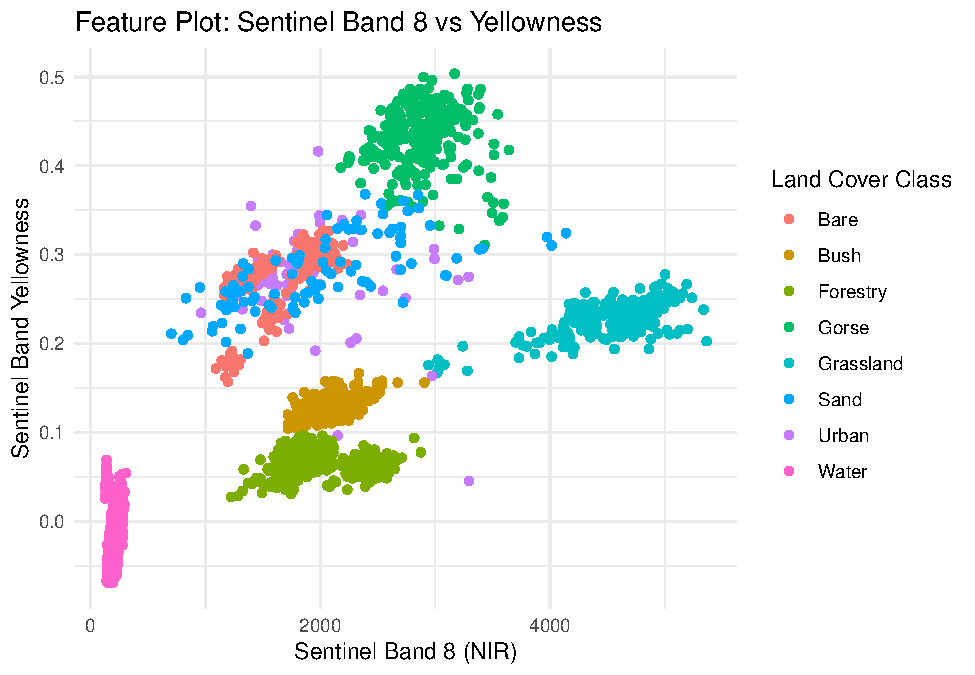
\includegraphics[keepaspectratio]{ML-based-modelling-for-spatial-and-spatiotemporal-data_files/figure-latex/featurePlot-1.pdf}}

The feature plot shows the distribution of training samples in the
feature space defined by Sentinel Band 8 (NIR) and the yellowness index.
It helps us visualize how well the different land cover classes can be
separated based on these features. The Gorse class features the highest
``yellowness'' values while all other land cover classes have
considerably lower values. Based on the feature plot, note that there is
only low separability considering Sentinel channel 3 and 4 (green and
red) but high separability when channel 8 (near infrared) or the
yellowness index is included.

\section{4. Machine Learning Model}\label{machine-learning-model}

The split data is now ready for training machine learning models and
ready for implementation in the three different algorithms:
\texttt{Random\ Forest}, \texttt{XGBoost}, and
\texttt{Support\ Vector\ Machine\ (SVM)}. Each model will be trained on
the training data set and evaluated on the test data set.

\textbf{Selecting predictor and response variable:} Before building the
ML models, all the Sentinel bands and indices were selected as the
predictor variables and the land cover class were selected as the
response variables. The response variable is categorical, while the
predictor variables are continuous. From the data, we select all the
information from the sentinel raster data as the predictor variables and
the land cover class as the response variable.

\begin{Shaded}
\begin{Highlighting}[]
\CommentTok{\# Select predictor variables (Sentinel bands and indices)}
\NormalTok{predictors }\OtherTok{\textless{}{-}} \FunctionTok{c}\NormalTok{(}\StringTok{"B02"}\NormalTok{, }\StringTok{"B03"}\NormalTok{, }\StringTok{"B04"}\NormalTok{, }\StringTok{"B05"}\NormalTok{, }\StringTok{"B06"}\NormalTok{, }\StringTok{"B07"}\NormalTok{, }\StringTok{"B08"}\NormalTok{, }\StringTok{"NDVI"}\NormalTok{, }\StringTok{"yellowness"}\NormalTok{)}

\CommentTok{\# Select response variable (land cover class)}
\NormalTok{response }\OtherTok{\textless{}{-}} \StringTok{\textquotesingle{}Class\textquotesingle{}}
\end{Highlighting}
\end{Shaded}

\subsection{Random Forest}\label{random-forest}

Random Forest is a popular ensemble learning method that constructs
multiple decision trees and merges them together to get a more accurate
and stable prediction. It is particularly effective for classification
tasks and suits this LC classification analysis. Training the Random
Forest model using the \texttt{randomForest} package in R. The model is
trained on the training data set, and we can visualize the variable
importance to understand which features contribute most to the
classification. We use the \texttt{train} function from the
\texttt{caret} package to train the model with 10-fold cross-validation
for hyperparameter tuning.

\begin{Shaded}
\begin{Highlighting}[]
\CommentTok{\# Ensure response is a factor}
\NormalTok{trainDat[, response] }\OtherTok{\textless{}{-}} \FunctionTok{as.factor}\NormalTok{(trainDat[, response])}

\CommentTok{\# Define hyperparameter tuning grid }
\NormalTok{rf\_grid }\OtherTok{\textless{}{-}} \FunctionTok{expand.grid}\NormalTok{(}
  \AttributeTok{mtry =} \FunctionTok{c}\NormalTok{(}\DecValTok{2}\NormalTok{, }\DecValTok{3}\NormalTok{, }\DecValTok{4}\NormalTok{),  }\CommentTok{\# Number of variables randomly sampled at each split}
  \AttributeTok{splitrule =} \StringTok{"gini"}\NormalTok{, }\CommentTok{\# Splitting rule}
  \AttributeTok{min.node.size =} \FunctionTok{c}\NormalTok{(}\DecValTok{1}\NormalTok{, }\DecValTok{5}\NormalTok{) }\CommentTok{\# Minimum size of terminal nodes}
\NormalTok{)}

\CommentTok{\# Setting train control}
\NormalTok{control }\OtherTok{\textless{}{-}} \FunctionTok{trainControl}\NormalTok{(}
  \AttributeTok{method =} \StringTok{"cv"}\NormalTok{,         }\CommentTok{\# k{-}fold CV}
  \AttributeTok{number =} \DecValTok{10}\NormalTok{,           }\CommentTok{\# 10{-}fold}
  \AttributeTok{summaryFunction =}\NormalTok{ multiClassSummary,  }\CommentTok{\# for multiclass metrics}
  \AttributeTok{classProbs =} \ConstantTok{TRUE}\NormalTok{,}
  \AttributeTok{savePredictions =} \StringTok{"final"}\NormalTok{,}
  \AttributeTok{sampling =} \StringTok{"up"}
\NormalTok{)}

\CommentTok{\# Train Random Forest model}
\FunctionTok{set.seed}\NormalTok{(}\DecValTok{100}\NormalTok{)}
\NormalTok{model\_rf }\OtherTok{\textless{}{-}} \FunctionTok{train}\NormalTok{(trainDat[, predictors], trainDat[, response], }
                  \AttributeTok{method =} \StringTok{"rf"}\NormalTok{, }
                  \AttributeTok{trControl =}\NormalTok{ control,}
                  \AttributeTok{importance =} \ConstantTok{TRUE}\NormalTok{)}
\end{Highlighting}
\end{Shaded}

\begin{Shaded}
\begin{Highlighting}[]
\CommentTok{\# Print model summary}
\FunctionTok{kable}\NormalTok{(model\_rf}\SpecialCharTok{$}\NormalTok{results, }\AttributeTok{caption =} \StringTok{"Random Forest Model Results"}\NormalTok{) }\SpecialCharTok{\%\textgreater{}\%}
  \FunctionTok{kable\_styling}\NormalTok{(}\AttributeTok{full\_width =}\NormalTok{ F, }\AttributeTok{position =} \StringTok{"left"}\NormalTok{)}
\end{Highlighting}
\end{Shaded}

\begin{longtable}[l]{rrrrrrrrrrrrrrrrrrrrrrrrrrrrr}
\caption{\label{tab:rf_summary}Random Forest Model Results}\\
\toprule
mtry & logLoss & AUC & prAUC & Accuracy & Kappa & Mean\_F1 & Mean\_Sensitivity & Mean\_Specificity & Mean\_Pos\_Pred\_Value & Mean\_Neg\_Pred\_Value & Mean\_Precision & Mean\_Recall & Mean\_Detection\_Rate & Mean\_Balanced\_Accuracy & logLossSD & AUCSD & prAUCSD & AccuracySD & KappaSD & Mean\_F1SD & Mean\_SensitivitySD & Mean\_SpecificitySD & Mean\_Pos\_Pred\_ValueSD & Mean\_Neg\_Pred\_ValueSD & Mean\_PrecisionSD & Mean\_RecallSD & Mean\_Detection\_RateSD & Mean\_Balanced\_AccuracySD\\
\midrule
2 & 0.0194079 & 0.9996537 & 0.3135054 & 0.9944470 & 0.9914640 & 0.9731647 & 0.9717758 & 0.9992815 & 0.9772389 & 0.9992905 & 0.9772389 & 0.9717758 & 0.1243059 & 0.9855286 & 0.0078280 & 0.0003859 & 0.0337306 & 0.0039935 & 0.0061337 & 0.0194530 & 0.0201904 & 0.0005168 & 0.0180031 & 0.0005101 & 0.0180031 & 0.0201904 & 0.0004992 & 0.0103524\\
5 & 0.0192705 & 0.9996919 & 0.2236961 & 0.9932740 & 0.9896542 & 0.9682776 & 0.9671660 & 0.9991251 & 0.9747691 & 0.9991392 & 0.9747691 & 0.9671660 & 0.1241592 & 0.9831455 & 0.0135754 & 0.0004931 & 0.0369808 & 0.0051617 & 0.0079476 & 0.0263027 & 0.0261678 & 0.0006728 & 0.0214679 & 0.0006581 & 0.0214679 & 0.0261678 & 0.0006452 & 0.0134152\\
9 & 0.0582227 & 0.9964809 & 0.1037647 & 0.9941511 & 0.9910037 & 0.9739457 & 0.9729646 & 0.9992407 & 0.9772993 & 0.9992473 & 0.9772993 & 0.9729646 & 0.1242689 & 0.9861027 & 0.0727093 & 0.0055828 & 0.0303429 & 0.0043519 & 0.0066949 & 0.0173850 & 0.0177504 & 0.0005681 & 0.0163332 & 0.0005644 & 0.0163332 & 0.0177504 & 0.0005440 & 0.0091501\\
\bottomrule
\end{longtable}

\begin{Shaded}
\begin{Highlighting}[]
\CommentTok{\# Extract variable importance}
\NormalTok{importance\_df }\OtherTok{\textless{}{-}} \FunctionTok{varImp}\NormalTok{(model\_rf)}\SpecialCharTok{$}\NormalTok{importance}

\CommentTok{\# Add variable names as a column}
\NormalTok{importance\_df}\SpecialCharTok{$}\NormalTok{Variable }\OtherTok{\textless{}{-}} \FunctionTok{rownames}\NormalTok{(importance\_df)}

\CommentTok{\# Compute overall importance (if multiple classes)}
\NormalTok{importance\_df}\SpecialCharTok{$}\NormalTok{Overall }\OtherTok{\textless{}{-}} \FunctionTok{rowMeans}\NormalTok{(importance\_df[, }\FunctionTok{sapply}\NormalTok{(importance\_df, is.numeric)])}

\CommentTok{\# Round and sort in descending order}
\NormalTok{importance\_df }\OtherTok{\textless{}{-}}\NormalTok{ importance\_df }\SpecialCharTok{\%\textgreater{}\%}
  \FunctionTok{mutate}\NormalTok{(}\AttributeTok{Overall =} \FunctionTok{round}\NormalTok{(Overall, }\DecValTok{3}\NormalTok{)) }\SpecialCharTok{\%\textgreater{}\%}
  \FunctionTok{arrange}\NormalTok{(}\FunctionTok{desc}\NormalTok{(Overall))  }\CommentTok{\# High to low}

\CommentTok{\# View top variables}
\FunctionTok{kable}\NormalTok{(importance\_df, }\AttributeTok{caption =} \StringTok{"Variable Importance for Random Forest Model"}\NormalTok{) }\SpecialCharTok{\%\textgreater{}\%}
  \FunctionTok{kable\_styling}\NormalTok{(}\AttributeTok{full\_width =}\NormalTok{ F, }\AttributeTok{position =} \StringTok{"left"}\NormalTok{)}
\end{Highlighting}
\end{Shaded}

\begin{longtable}[l]{lrrrrrrrrlr}
\caption{\label{tab:rf_summary}Variable Importance for Random Forest Model}\\
\toprule
 & Bare & Bush & Forestry & Gorse & Grassland & Sand & Urban & Water & Variable & Overall\\
\midrule
NDVI & 78.81922 & 51.74690 & 42.84082 & 67.26438 & 54.32107 & 82.43570 & 96.46106 & 27.60330 & NDVI & 62.687\\
yellowness & 80.57554 & 44.51956 & 41.20206 & 75.49890 & 40.48474 & 53.72358 & 82.26013 & 20.75973 & yellowness & 54.878\\
B05 & 57.84457 & 41.90438 & 38.77014 & 43.10041 & 40.90441 & 99.16067 & 79.66702 & 33.45632 & B05 & 54.351\\
B07 & 70.04270 & 42.26636 & 33.83277 & 42.12963 & 35.77620 & 64.99589 & 84.73350 & 29.86652 & B07 & 50.455\\
B06 & 65.81163 & 41.86432 & 32.35504 & 40.79115 & 30.54126 & 64.34196 & 84.33848 & 34.24737 & B06 & 49.286\\
\addlinespace
B04 & 59.79071 & 51.15562 & 31.61819 & 54.23198 & 30.60026 & 64.23863 & 77.03137 & 21.19083 & B04 & 48.732\\
B02 & 93.18263 & 19.81698 & 15.63798 & 57.58772 & 16.88825 & 67.45459 & 100.00000 & 14.20616 & B02 & 48.097\\
B08 & 54.83551 & 37.96788 & 31.79415 & 32.47370 & 29.06082 & 67.23859 & 92.70732 & 31.65667 & B08 & 47.217\\
B03 & 70.19851 & 36.28995 & 41.09424 & 45.42369 & 33.77928 & 65.11085 & 72.26431 & 0.00000 & B03 & 45.520\\
\bottomrule
\end{longtable}

\begin{Shaded}
\begin{Highlighting}[]
\CommentTok{\# Plot variable importance}
\FunctionTok{ggplot}\NormalTok{(importance\_df, }\FunctionTok{aes}\NormalTok{(}\AttributeTok{x =} \FunctionTok{reorder}\NormalTok{(Variable, Overall), }\AttributeTok{y =}\NormalTok{ Overall)) }\SpecialCharTok{+}
  \FunctionTok{geom\_bar}\NormalTok{(}\AttributeTok{stat =} \StringTok{"identity"}\NormalTok{, }\AttributeTok{fill =} \StringTok{"steelblue"}\NormalTok{) }\SpecialCharTok{+}
  \FunctionTok{coord\_flip}\NormalTok{() }\SpecialCharTok{+}
  \FunctionTok{labs}\NormalTok{(}\AttributeTok{title =} \StringTok{"Variable Importance for RF model (High to Low)"}\NormalTok{,}
       \AttributeTok{x =} \StringTok{"Variable"}\NormalTok{, }\AttributeTok{y =} \StringTok{"Importance Score"}\NormalTok{) }\SpecialCharTok{+}
  \FunctionTok{theme\_minimal}\NormalTok{()}
\end{Highlighting}
\end{Shaded}

\pandocbounded{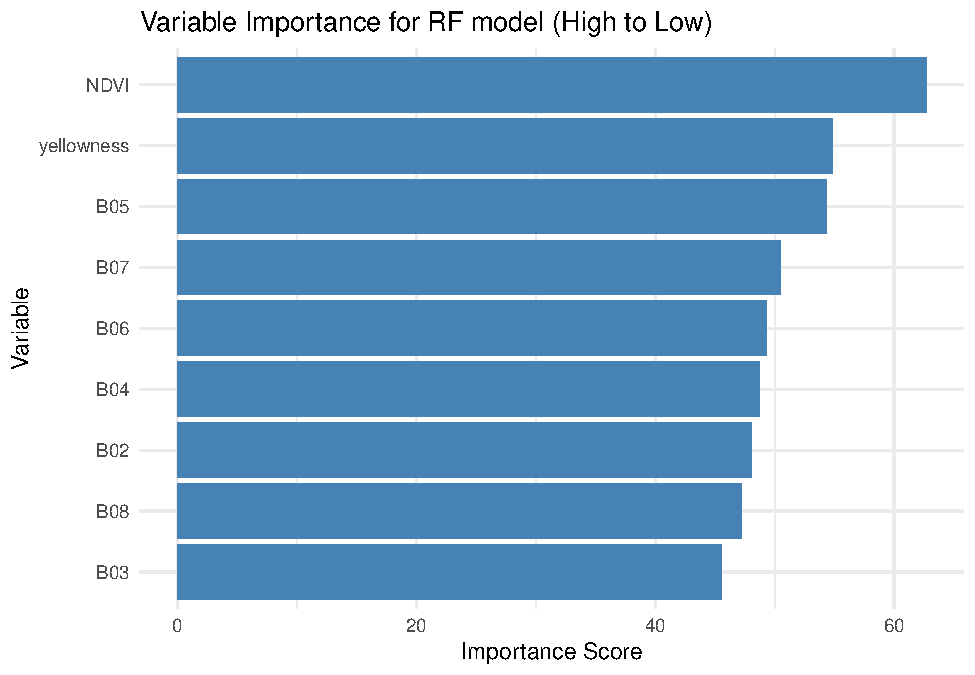
\includegraphics[keepaspectratio]{ML-based-modelling-for-spatial-and-spatiotemporal-data_files/figure-latex/rf_summary-1.pdf}}

The Random Forest model is successfully trained and variable importance
is noted for the determining which predictor variable (sentinel bands)
has overall contributions to the classification. The model achieved
excellent performance across multiple values of \texttt{mtry}, with the
least logLoss results at 5. At \texttt{mtry} at 5, the model shows,

\begin{itemize}
\item
  Least uncertainity (\emph{logLoss = 0.0192}),
\item
  Nearly perfect classification (\emph{AUC score = 0.999}),
\item
  High classification (\emph{accuracy = 0.9933}),
\item
  Good overall class performance (\emph{balanced accuracy = 0.9831}) and
\item
  Balanced precision and recall (\emph{mean F1 score = 0.968}).
\end{itemize}

The variable importance scores for each predictor variable is derived.
The variable importance plot shows which features contribute most to the
classification task, with the \texttt{NDVI}, \texttt{Yellowness} \&
\texttt{B05} being among the top 3 important predictors.

\textbf{Predicting the test data with confusion matrix and scoring
metrics:} To evaluate the performance of the Random Forest model on the
test data set, we can create a confusion matrix and calculate scoring
metrics such as accuracy, sensitivity, and specificity. The confusion
matrix provides insights into how well the model performs on the test
data set.

\begin{Shaded}
\begin{Highlighting}[]
\CommentTok{\# Predict on the test dataset}
\NormalTok{predictions\_rf }\OtherTok{\textless{}{-}} \FunctionTok{predict}\NormalTok{(model\_rf,}
                          \AttributeTok{newdata =}\NormalTok{ testDat[, predictors])}

\CommentTok{\# Extract the levels from the training data response}
\NormalTok{true\_levels }\OtherTok{\textless{}{-}} \FunctionTok{levels}\NormalTok{(trainDat[[response]])}

\CommentTok{\# Convert both predicted and actual responses to factors with the same levels}
\NormalTok{predictions\_rf }\OtherTok{\textless{}{-}} \FunctionTok{factor}\NormalTok{(predictions\_rf, }\AttributeTok{levels =}\NormalTok{ true\_levels)}
\NormalTok{actual\_rf }\OtherTok{\textless{}{-}} \FunctionTok{factor}\NormalTok{(testDat[[response]], }\AttributeTok{levels =}\NormalTok{ true\_levels)}

\CommentTok{\# Construct the confusion matrix}
\NormalTok{confusion\_rf }\OtherTok{\textless{}{-}}\NormalTok{ caret}\SpecialCharTok{::}\FunctionTok{confusionMatrix}\NormalTok{(predictions\_rf, actual\_rf)}

\CommentTok{\# Plot confusion matrix}
\NormalTok{cm\_plot\_rf }\OtherTok{\textless{}{-}} \FunctionTok{ggplot}\NormalTok{(}\FunctionTok{as.data.frame}\NormalTok{(confusion\_rf}\SpecialCharTok{$}\NormalTok{table), }
                     \FunctionTok{aes}\NormalTok{(}\AttributeTok{x =}\NormalTok{ Reference, }\AttributeTok{y =}\NormalTok{ Prediction)) }\SpecialCharTok{+}
  \FunctionTok{geom\_tile}\NormalTok{(}\FunctionTok{aes}\NormalTok{(}\AttributeTok{fill =}\NormalTok{ Freq), }\AttributeTok{color =} \StringTok{"white"}\NormalTok{) }\SpecialCharTok{+}
  \FunctionTok{scale\_fill\_gradient}\NormalTok{(}\AttributeTok{low =} \StringTok{"white"}\NormalTok{, }\AttributeTok{high =} \StringTok{"steelblue"}\NormalTok{) }\SpecialCharTok{+}
  \FunctionTok{geom\_text}\NormalTok{(}\FunctionTok{aes}\NormalTok{(}\AttributeTok{label =}\NormalTok{ Freq), }\AttributeTok{color =} \StringTok{"black"}\NormalTok{) }\SpecialCharTok{+}
  \FunctionTok{labs}\NormalTok{(}\AttributeTok{title =} \StringTok{"Confusion Matrix for Random Forest Model"}\NormalTok{,}
       \AttributeTok{x =} \StringTok{"Reference Class"}\NormalTok{,}
       \AttributeTok{y =} \StringTok{"Predicted Class"}\NormalTok{) }\SpecialCharTok{+}
  \FunctionTok{theme\_minimal}\NormalTok{() }\SpecialCharTok{+}
  \FunctionTok{theme}\NormalTok{(}\AttributeTok{axis.text.x =} \FunctionTok{element\_text}\NormalTok{(}\AttributeTok{angle =} \DecValTok{45}\NormalTok{, }\AttributeTok{hjust =} \DecValTok{1}\NormalTok{))}

\NormalTok{cm\_plot\_rf}
\end{Highlighting}
\end{Shaded}

\pandocbounded{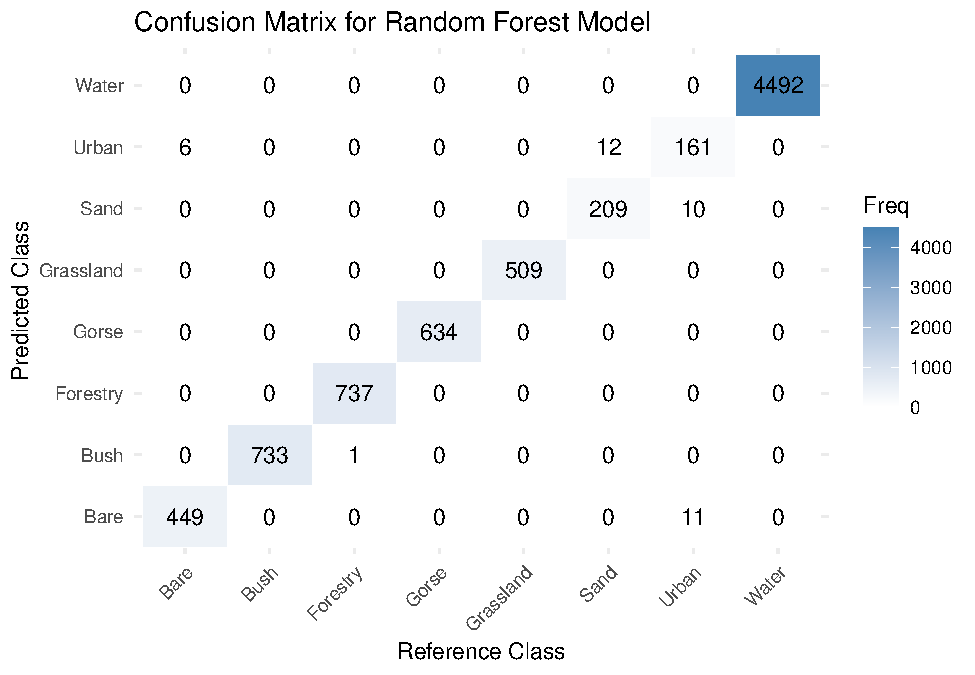
\includegraphics[keepaspectratio]{ML-based-modelling-for-spatial-and-spatiotemporal-data_files/figure-latex/rf_confusion_matrix-1.pdf}}

\begin{Shaded}
\begin{Highlighting}[]
\CommentTok{\# Print scoring metrics}
\FunctionTok{kable}\NormalTok{(confusion\_rf}\SpecialCharTok{$}\NormalTok{overall, }\AttributeTok{caption =} \StringTok{"Scoring Metrics for Random Forest Model"}\NormalTok{) }\SpecialCharTok{\%\textgreater{}\%}
  \FunctionTok{kable\_styling}\NormalTok{(}\AttributeTok{full\_width =}\NormalTok{ F, }\AttributeTok{position =} \StringTok{"left"}\NormalTok{)}
\end{Highlighting}
\end{Shaded}

\begin{longtable}[l]{lr}
\caption{\label{tab:rf_confusion_matrix}Scoring Metrics for Random Forest Model}\\
\toprule
 & x\\
\midrule
Accuracy & 0.9949774\\
Kappa & 0.9922706\\
AccuracyLower & 0.9931669\\
AccuracyUpper & 0.9964094\\
AccuracyNull & 0.5640382\\
\addlinespace
AccuracyPValue & 0.0000000\\
McnemarPValue & NaN\\
\bottomrule
\end{longtable}

\begin{Shaded}
\begin{Highlighting}[]
\CommentTok{\# Print sensitivity and specificity for each class}
\FunctionTok{kable}\NormalTok{(confusion\_rf}\SpecialCharTok{$}\NormalTok{byClass, }\AttributeTok{caption =} \StringTok{"Sensitivity and Specificity for Random Forest Model"}\NormalTok{) }\SpecialCharTok{\%\textgreater{}\%}
  \FunctionTok{kable\_styling}\NormalTok{(}\AttributeTok{full\_width =}\NormalTok{ F, }\AttributeTok{position =} \StringTok{"left"}\NormalTok{)}
\end{Highlighting}
\end{Shaded}

\begin{longtable}[l]{lrrrrrrrrrrr}
\caption{\label{tab:rf_confusion_matrix}Sensitivity and Specificity for Random Forest Model}\\
\toprule
 & Sensitivity & Specificity & Pos Pred Value & Neg Pred Value & Precision & Recall & F1 & Prevalence & Detection Rate & Detection Prevalence & Balanced Accuracy\\
\midrule
Class: Bare & 0.9868132 & 0.9985351 & 0.9760870 & 0.9992004 & 0.9760870 & 0.9868132 & 0.9814208 & 0.0571321 & 0.0563787 & 0.0577599 & 0.9926741\\
Class: Bush & 1.0000000 & 0.9998617 & 0.9986376 & 1.0000000 & 0.9986376 & 1.0000000 & 0.9993183 & 0.0920392 & 0.0920392 & 0.0921647 & 0.9999309\\
Class: Forestry & 0.9986450 & 1.0000000 & 1.0000000 & 0.9998616 & 1.0000000 & 0.9986450 & 0.9993220 & 0.0926670 & 0.0925414 & 0.0925414 & 0.9993225\\
Class: Gorse & 1.0000000 & 1.0000000 & 1.0000000 & 1.0000000 & 1.0000000 & 1.0000000 & 1.0000000 & 0.0796082 & 0.0796082 & 0.0796082 & 1.0000000\\
Class: Grassland & 1.0000000 & 1.0000000 & 1.0000000 & 1.0000000 & 1.0000000 & 1.0000000 & 1.0000000 & 0.0639126 & 0.0639126 & 0.0639126 & 1.0000000\\
\addlinespace
Class: Sand & 0.9457014 & 0.9987085 & 0.9543379 & 0.9984506 & 0.9543379 & 0.9457014 & 0.9500000 & 0.0277499 & 0.0262431 & 0.0274987 & 0.9722049\\
Class: Urban & 0.8846154 & 0.9976870 & 0.8994413 & 0.9973025 & 0.8994413 & 0.8846154 & 0.8919668 & 0.0228528 & 0.0202160 & 0.0224761 & 0.9411512\\
Class: Water & 1.0000000 & 1.0000000 & 1.0000000 & 1.0000000 & 1.0000000 & 1.0000000 & 1.0000000 & 0.5640382 & 0.5640382 & 0.5640382 & 1.0000000\\
\bottomrule
\end{longtable}

\textbf{Results:} Confusion Matrix and scoring metrics provide insights
into the performance of the Random Forest model on the test data set.
The confusion matrix shows how many instances were correctly classified
for each land cover class, while the scoring metrics (accuracy,
sensitivity, specificity) quantify the model's overall performance.

Predictions on the test/unseen data, confusion matrix shows high true
positives for all the classes predictions with an overall accuracy of
99.5\%, but do have some irregularities in the classification. From the
confusion matrix,

\begin{itemize}
\item
  \texttt{Water}, \texttt{Grassland}, \texttt{Gorse}, \& \texttt{Bush}
  are 100\% predicted and classified correctly.
\item
  Out of 738 \texttt{Forestry} Class, 1 was predicted as Bush
\item
  Out of 182 \texttt{Urban} Class, 10 were predicted as \texttt{Sand}
  and 11 as \texttt{Bare}.
\item
  Out of 221 \texttt{Sand} Class, 12 were predicted as \texttt{Urban}.
\item
  Out of 455 \texttt{Bare} class, 6 were predicted as \texttt{Urban}.
\end{itemize}

This means that the \texttt{Urban}, \texttt{Bare} and \texttt{Sand} show
very little false positives with the RF model.

\subsection{XGBoost (Extreme Gradient Boosting)}\label{xgboost}

XGBoost (Extreme Gradient Boosting) is a powerful and efficient
implementation of gradient boosting that is widely used for
classification tasks. It is known for its speed and performance, making
it suitable for large data sets. Training the XGBoost model using the
\texttt{xgboost} package in R. The model is trained on the training data
set, and we can visualize the variable importance to understand which
features contribute most to the classification. We use the
\texttt{train} function from the \texttt{caret} package to train the
model with 10-fold cross-validation for hyperparameter tuning.

\begin{Shaded}
\begin{Highlighting}[]
\CommentTok{\# Ensure response is a factor}
\NormalTok{trainDat[, response] }\OtherTok{\textless{}{-}} \FunctionTok{as.factor}\NormalTok{(trainDat[, response])}

\CommentTok{\# Define hyperparameter tuning grid }
\NormalTok{xgb\_grid }\OtherTok{\textless{}{-}} \FunctionTok{expand.grid}\NormalTok{(}
  \AttributeTok{nrounds =} \DecValTok{100}\NormalTok{,}
  \AttributeTok{max\_depth =} \DecValTok{6}\NormalTok{,}
  \AttributeTok{eta =} \FloatTok{0.3}\NormalTok{,}
  \AttributeTok{gamma =} \DecValTok{0}\NormalTok{,}
  \AttributeTok{colsample\_bytree =} \DecValTok{1}\NormalTok{,}
  \AttributeTok{min\_child\_weight =} \DecValTok{1}\NormalTok{,}
  \AttributeTok{subsample =} \DecValTok{1}
\NormalTok{)}

\CommentTok{\# Setting train control}
\NormalTok{control }\OtherTok{\textless{}{-}} \FunctionTok{trainControl}\NormalTok{(}
  \AttributeTok{method =} \StringTok{"cv"}\NormalTok{,         }\CommentTok{\# k{-}fold CV}
  \AttributeTok{number =} \DecValTok{10}\NormalTok{,           }\CommentTok{\# 10{-}fold}
  \AttributeTok{summaryFunction =}\NormalTok{ multiClassSummary,  }\CommentTok{\# for multiclass metrics}
  \AttributeTok{classProbs =} \ConstantTok{TRUE}\NormalTok{,}
  \AttributeTok{savePredictions =} \StringTok{"final"}\NormalTok{,}
  \AttributeTok{sampling =} \StringTok{"up"}\NormalTok{,}
  \AttributeTok{verboseIter =} \ConstantTok{FALSE}
\NormalTok{)}

\CommentTok{\# Train the XGBoost model using caret}
\FunctionTok{set.seed}\NormalTok{(}\DecValTok{100}\NormalTok{)}
\NormalTok{model\_xgb }\OtherTok{\textless{}{-}} \FunctionTok{train}\NormalTok{(}\AttributeTok{x =}\NormalTok{ trainDat[, predictors],}
                   \AttributeTok{y =}\NormalTok{ trainDat[, response],}
                   \AttributeTok{method =} \StringTok{"xgbTree"}\NormalTok{,}
                   \AttributeTok{trControl =}\NormalTok{ control,}
                   \AttributeTok{tuneGrid =}\NormalTok{ xgb\_grid)}
\end{Highlighting}
\end{Shaded}

\begin{Shaded}
\begin{Highlighting}[]
\CommentTok{\# Print model summary}
\FunctionTok{kable}\NormalTok{(model\_xgb}\SpecialCharTok{$}\NormalTok{results, }\AttributeTok{caption =} \StringTok{"XGBoost Model Results"}\NormalTok{) }\SpecialCharTok{\%\textgreater{}\%}
  \FunctionTok{kable\_styling}\NormalTok{(}\AttributeTok{full\_width =}\NormalTok{ F, }\AttributeTok{position =} \StringTok{"left"}\NormalTok{)}
\end{Highlighting}
\end{Shaded}

\begin{longtable}[l]{rrrrrrrrrrrrrrrrrrrrrrrrrrrrrrrrrrr}
\caption{\label{tab:xgb_summary}XGBoost Model Results}\\
\toprule
nrounds & max\_depth & eta & gamma & colsample\_bytree & min\_child\_weight & subsample & logLoss & AUC & prAUC & Accuracy & Kappa & Mean\_F1 & Mean\_Sensitivity & Mean\_Specificity & Mean\_Pos\_Pred\_Value & Mean\_Neg\_Pred\_Value & Mean\_Precision & Mean\_Recall & Mean\_Detection\_Rate & Mean\_Balanced\_Accuracy & logLossSD & AUCSD & prAUCSD & AccuracySD & KappaSD & Mean\_F1SD & Mean\_SensitivitySD & Mean\_SpecificitySD & Mean\_Pos\_Pred\_ValueSD & Mean\_Neg\_Pred\_ValueSD & Mean\_PrecisionSD & Mean\_RecallSD & Mean\_Detection\_RateSD & Mean\_Balanced\_AccuracySD\\
\midrule
100 & 6 & 0.3 & 0 & 1 & 1 & 1 & 0.0283113 & 0.9997245 & 0.8622213 & 0.9929867 & 0.9892228 & 0.9708748 & 0.9697435 & 0.9990861 & 0.9750296 & 0.9990923 & 0.9750296 & 0.9697435 & 0.1241233 & 0.9844148 & 0.0222191 & 0.000436 & 0.0349824 & 0.0047978 & 0.0073673 & 0.0198403 & 0.0213631 & 0.0006256 & 0.015926 & 0.000619 & 0.015926 & 0.0213631 & 0.0005997 & 0.0109808\\
\bottomrule
\end{longtable}

\begin{Shaded}
\begin{Highlighting}[]
\CommentTok{\# Extract variable importance}
\NormalTok{importance\_xgb }\OtherTok{\textless{}{-}} \FunctionTok{xgb.importance}\NormalTok{(}\AttributeTok{feature\_names =}\NormalTok{ predictors, }
                                 \AttributeTok{model =}\NormalTok{ model\_xgb}\SpecialCharTok{$}\NormalTok{finalModel)}

\CommentTok{\# Convert importance to a data frame}
\NormalTok{importance\_df\_xgb }\OtherTok{\textless{}{-}} \FunctionTok{as.data.frame}\NormalTok{(importance\_xgb)}
\NormalTok{importance\_df\_xgb }\OtherTok{\textless{}{-}}\NormalTok{ importance\_df\_xgb }\SpecialCharTok{\%\textgreater{}\%}
  \FunctionTok{mutate}\NormalTok{(}\AttributeTok{Variable =} \FunctionTok{reorder}\NormalTok{(Feature, Gain)) }\SpecialCharTok{\%\textgreater{}\%}
  \FunctionTok{arrange}\NormalTok{(}\FunctionTok{desc}\NormalTok{(Gain))}

\CommentTok{\# Check the summary of the importance data frame}
\FunctionTok{kable}\NormalTok{(importance\_df\_xgb, }\AttributeTok{caption =} \StringTok{"Variable Importance for XGBoost Model"}\NormalTok{) }\SpecialCharTok{\%\textgreater{}\%}
  \FunctionTok{kable\_styling}\NormalTok{(}\AttributeTok{full\_width =}\NormalTok{ F, }\AttributeTok{position =} \StringTok{"left"}\NormalTok{)}
\end{Highlighting}
\end{Shaded}

\begin{longtable}[l]{lrrrl}
\caption{\label{tab:xgb_summary}Variable Importance for XGBoost Model}\\
\toprule
Feature & Gain & Cover & Frequency & Variable\\
\midrule
B05 & 0.2319615 & 0.1726225 & 0.1417647 & B05\\
yellowness & 0.1889079 & 0.1664336 & 0.1629412 & yellowness\\
B02 & 0.1794137 & 0.1838177 & 0.1776471 & B02\\
B03 & 0.1585555 & 0.1987152 & 0.1423529 & B03\\
B07 & 0.1433434 & 0.1102423 & 0.1052941 & B07\\
\addlinespace
B04 & 0.0420511 & 0.1087894 & 0.0747059 & B04\\
NDVI & 0.0339618 & 0.0339363 & 0.0970588 & NDVI\\
B06 & 0.0186276 & 0.0191703 & 0.0582353 & B06\\
B08 & 0.0031775 & 0.0062727 & 0.0400000 & B08\\
\bottomrule
\end{longtable}

\begin{Shaded}
\begin{Highlighting}[]
\CommentTok{\# Visualize variable importance using ggplot2}
\FunctionTok{ggplot}\NormalTok{(importance\_df\_xgb, }\FunctionTok{aes}\NormalTok{(}\AttributeTok{x =}\NormalTok{ Variable, }\AttributeTok{y =}\NormalTok{ Gain)) }\SpecialCharTok{+}
  \FunctionTok{geom\_bar}\NormalTok{(}\AttributeTok{stat =} \StringTok{"identity"}\NormalTok{, }\AttributeTok{fill =} \StringTok{"steelblue"}\NormalTok{) }\SpecialCharTok{+}
  \FunctionTok{coord\_flip}\NormalTok{() }\SpecialCharTok{+}
  \FunctionTok{labs}\NormalTok{(}\AttributeTok{title =} \StringTok{"Variable Importance for XGBoost (High to Low)"}\NormalTok{,}
       \AttributeTok{x =} \StringTok{"Variable"}\NormalTok{, }\AttributeTok{y =} \StringTok{"Importance Score"}\NormalTok{) }\SpecialCharTok{+}
  \FunctionTok{theme\_minimal}\NormalTok{()}
\end{Highlighting}
\end{Shaded}

\pandocbounded{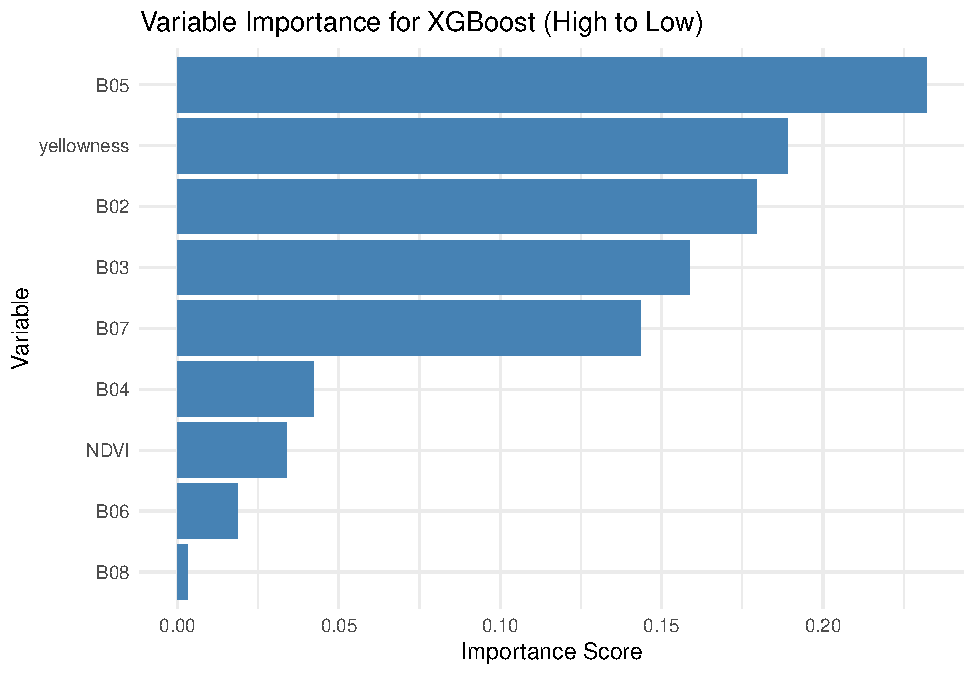
\includegraphics[keepaspectratio]{ML-based-modelling-for-spatial-and-spatiotemporal-data_files/figure-latex/xgb_summary-1.pdf}}

The XGBoost model is successfully trained and variable importance is
noted for the determining which predictor variable (sentinel bands) has
overall contributions to the classification. The variable importance
scores for each predictor variable is derived. The variable importance
plot shows which features contribute most to the classification task,
with the \texttt{B05}, \texttt{Yellowness} \& \texttt{B02} being among
the top 3 important predictors for the XGBoost model.

The XGBoost model has been trained successfully with the selected
hyperparameter. The model achieved excellent performance having,

\begin{itemize}
\item
  Least uncertainity (\emph{logLoss = 0.0283}),
\item
  Nearly perfect classification (\emph{AUC score = 0.999}),
\item
  Perfect agreement beyond chance (\emph{Kappa = 0.989}),
\item
  High classification (\emph{Accuracy = 0.993}),
\item
  Good overall class performance (\emph{balanced accuracy = 0.984}), and
\item
  Balanced precision and recall (\emph{mean F1 score = 0.97}).
\end{itemize}

These score are very similar to the Random Forest Model and will be
compared in the results and discussion section.

\textbf{Predicting the test data with confusion matrix and scoring
metrics:} To evaluate the performance of the XGBoost model on the test
data set, we can create a confusion matrix and calculate scoring metrics
such as accuracy, sensitivity, and specificity. The confusion matrix
provides insights into how well the model performs on the test data set.

\begin{Shaded}
\begin{Highlighting}[]
\CommentTok{\# Predict on the test dataset}
\NormalTok{predictions\_xgb }\OtherTok{\textless{}{-}} \FunctionTok{predict}\NormalTok{(model\_xgb, }\AttributeTok{newdata =}\NormalTok{ testDat[, predictors])}

\CommentTok{\# Extract the levels from the training data response}
\NormalTok{true\_levels\_xgb }\OtherTok{\textless{}{-}} \FunctionTok{levels}\NormalTok{(trainDat[[response]])}

\CommentTok{\# Convert both predicted and actual responses to factors with the same levels}
\NormalTok{predictions\_xgb }\OtherTok{\textless{}{-}} \FunctionTok{factor}\NormalTok{(predictions\_xgb, }\AttributeTok{levels =}\NormalTok{ true\_levels\_xgb)}
\NormalTok{actual\_xgb }\OtherTok{\textless{}{-}} \FunctionTok{factor}\NormalTok{(testDat[[response]], }\AttributeTok{levels =}\NormalTok{ true\_levels\_xgb)}

\CommentTok{\# Now create the confusion matrix}
\NormalTok{confusion\_xgb }\OtherTok{\textless{}{-}}\NormalTok{ caret}\SpecialCharTok{::}\FunctionTok{confusionMatrix}\NormalTok{(predictions\_xgb, actual\_xgb)}

\CommentTok{\# Plot confusion matrix}
\NormalTok{cm\_plot\_xgb }\OtherTok{\textless{}{-}} \FunctionTok{ggplot}\NormalTok{(}\FunctionTok{as.data.frame}\NormalTok{(confusion\_xgb}\SpecialCharTok{$}\NormalTok{table), }\FunctionTok{aes}\NormalTok{(}\AttributeTok{x =}\NormalTok{ Reference, }\AttributeTok{y =}\NormalTok{ Prediction)) }\SpecialCharTok{+}
  \FunctionTok{geom\_tile}\NormalTok{(}\FunctionTok{aes}\NormalTok{(}\AttributeTok{fill =}\NormalTok{ Freq), }\AttributeTok{color =} \StringTok{"white"}\NormalTok{) }\SpecialCharTok{+}
  \FunctionTok{scale\_fill\_gradient}\NormalTok{(}\AttributeTok{low =} \StringTok{"white"}\NormalTok{, }\AttributeTok{high =} \StringTok{"steelblue"}\NormalTok{) }\SpecialCharTok{+}
  \FunctionTok{geom\_text}\NormalTok{(}\FunctionTok{aes}\NormalTok{(}\AttributeTok{label =}\NormalTok{ Freq), }\AttributeTok{color =} \StringTok{"black"}\NormalTok{) }\SpecialCharTok{+}
  \FunctionTok{labs}\NormalTok{(}\AttributeTok{title =} \StringTok{"Confusion Matrix for XGBoost Model"}\NormalTok{,}
       \AttributeTok{x =} \StringTok{"Reference Class"}\NormalTok{,}
       \AttributeTok{y =} \StringTok{"Predicted Class"}\NormalTok{) }\SpecialCharTok{+}
  \FunctionTok{theme\_minimal}\NormalTok{() }\SpecialCharTok{+}
  \FunctionTok{theme}\NormalTok{(}\AttributeTok{axis.text.x =} \FunctionTok{element\_text}\NormalTok{(}\AttributeTok{angle =} \DecValTok{45}\NormalTok{, }\AttributeTok{hjust =} \DecValTok{1}\NormalTok{))}

\NormalTok{cm\_plot\_xgb}
\end{Highlighting}
\end{Shaded}

\pandocbounded{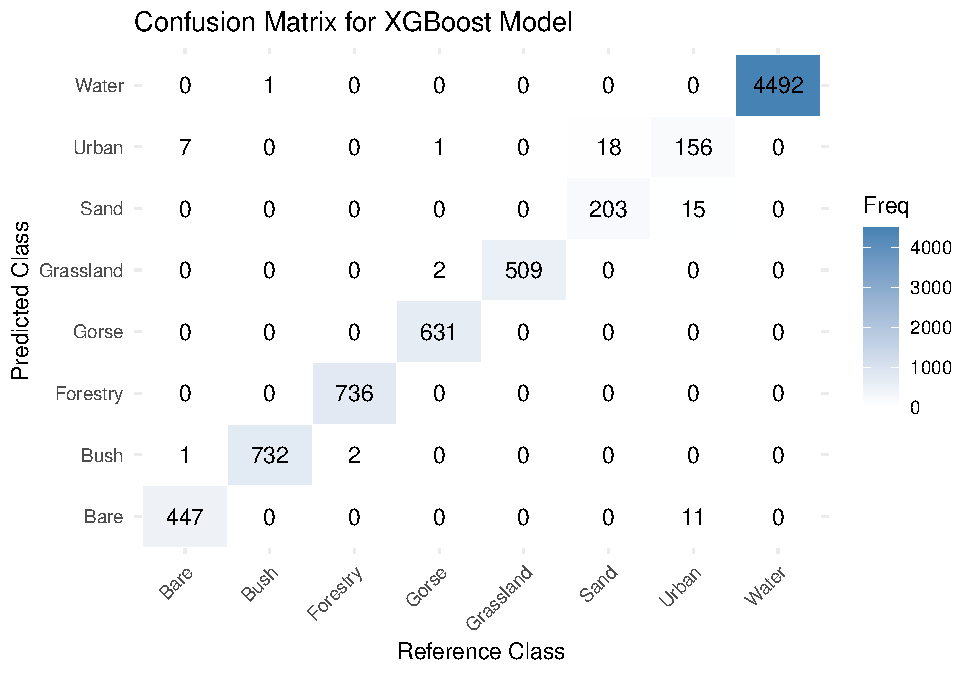
\includegraphics[keepaspectratio]{ML-based-modelling-for-spatial-and-spatiotemporal-data_files/figure-latex/xgb_confusion_matrix-1.pdf}}

\begin{Shaded}
\begin{Highlighting}[]
\CommentTok{\# Print scoring metrics}
\FunctionTok{kable}\NormalTok{(confusion\_xgb}\SpecialCharTok{$}\NormalTok{overall, }\AttributeTok{caption =} \StringTok{"Scoring Metrics for XGBoost Model"}\NormalTok{) }\SpecialCharTok{\%\textgreater{}\%} 
  \FunctionTok{kable\_styling}\NormalTok{(}\AttributeTok{full\_width =}\NormalTok{ F, }\AttributeTok{position =} \StringTok{"left"}\NormalTok{)}
\end{Highlighting}
\end{Shaded}

\begin{longtable}[l]{lr}
\caption{\label{tab:xgb_confusion_matrix}Scoring Metrics for XGBoost Model}\\
\toprule
 & x\\
\midrule
Accuracy & 0.9927172\\
Kappa & 0.9887915\\
AccuracyLower & 0.9905954\\
AccuracyUpper & 0.9944654\\
AccuracyNull & 0.5640382\\
\addlinespace
AccuracyPValue & 0.0000000\\
McnemarPValue & NaN\\
\bottomrule
\end{longtable}

\begin{Shaded}
\begin{Highlighting}[]
\CommentTok{\# Print sensitivity and specificity for each class}
\FunctionTok{kable}\NormalTok{(confusion\_xgb}\SpecialCharTok{$}\NormalTok{byClass, }\AttributeTok{caption =} \StringTok{"Sensitivity and Specificity for XGBoost Model"}\NormalTok{) }\SpecialCharTok{\%\textgreater{}\%} 
  \FunctionTok{kable\_styling}\NormalTok{(}\AttributeTok{full\_width =}\NormalTok{ F, }\AttributeTok{position =} \StringTok{"left"}\NormalTok{)}
\end{Highlighting}
\end{Shaded}

\begin{longtable}[l]{lrrrrrrrrrrr}
\caption{\label{tab:xgb_confusion_matrix}Sensitivity and Specificity for XGBoost Model}\\
\toprule
 & Sensitivity & Specificity & Pos Pred Value & Neg Pred Value & Precision & Recall & F1 & Prevalence & Detection Rate & Detection Prevalence & Balanced Accuracy\\
\midrule
Class: Bare & 0.9824176 & 0.9985351 & 0.9759825 & 0.9989342 & 0.9759825 & 0.9824176 & 0.9791895 & 0.0571321 & 0.0561276 & 0.0575088 & 0.9904763\\
Class: Bush & 0.9986357 & 0.9995851 & 0.9959184 & 0.9998617 & 0.9959184 & 0.9986357 & 0.9972752 & 0.0920392 & 0.0919136 & 0.0922903 & 0.9991104\\
Class: Forestry & 0.9972900 & 1.0000000 & 1.0000000 & 0.9997233 & 1.0000000 & 0.9972900 & 0.9986431 & 0.0926670 & 0.0924159 & 0.0924159 & 0.9986450\\
Class: Gorse & 0.9952681 & 1.0000000 & 1.0000000 & 0.9995909 & 1.0000000 & 0.9952681 & 0.9976285 & 0.0796082 & 0.0792315 & 0.0792315 & 0.9976341\\
Class: Grassland & 1.0000000 & 0.9997317 & 0.9960861 & 1.0000000 & 0.9960861 & 1.0000000 & 0.9980392 & 0.0639126 & 0.0639126 & 0.0641637 & 0.9998659\\
\addlinespace
Class: Sand & 0.9185520 & 0.9980628 & 0.9311927 & 0.9976762 & 0.9311927 & 0.9185520 & 0.9248292 & 0.0277499 & 0.0254897 & 0.0273732 & 0.9583074\\
Class: Urban & 0.8571429 & 0.9966590 & 0.8571429 & 0.9966590 & 0.8571429 & 0.8571429 & 0.8571429 & 0.0228528 & 0.0195881 & 0.0228528 & 0.9269009\\
Class: Water & 1.0000000 & 0.9997120 & 0.9997774 & 1.0000000 & 0.9997774 & 1.0000000 & 0.9998887 & 0.5640382 & 0.5640382 & 0.5641637 & 0.9998560\\
\bottomrule
\end{longtable}

\textbf{Results} Confusion Matrix and scoring metrics provide insights
into the performance of the XGBoost model on the test dataset. The
confusion matrix shows how many instances were correctly classified for
each land cover class, while the scoring metrics (accuracy, sensitivity,
specificity) quantify the model's overall performance.

Predictions on the test/unseen data for the XGBoost model, confusion
matrix shows high true positives for all the classes predictions with an
overall accuracy of 99.27\%, but do have some irregularities in the
classification. From the confusion matrix,

\begin{itemize}
\item
  \texttt{Water}, \texttt{Grassland}, \& \texttt{Forestry} are 100\%
  predicted and classified correctly.
\item
  Out of 182 \texttt{Urban} Class, 15 were predicted as \texttt{Sand}
  and 11 as \texttt{Bare}
\item
  Out of 221 \texttt{Sand} Class, 18 were predicted as \texttt{Urban}
\item
  Out of 634 \texttt{Gorse} Class, 2 were predicted as
  \texttt{Grassland} and 1 as Urban
\item
  Out of 733 \texttt{Bush} Class, 1 was predicted as \texttt{Water}
\item
  Out of 455 \texttt{Bare} class, 7 were predicted as \texttt{Urban} and
  1 as \texttt{Bush}.
\end{itemize}

This means that the \texttt{Urban}, \texttt{Sand}, \texttt{Gorse},
\texttt{Bush} and \texttt{Bare} show little false positives with the
XGBoost model.

\subsection{Support Vector Machine
(SVM)}\label{support-vector-machine-svm}

Support Vector Machine (SVM) is a supervised learning algorithm that can
be used for classification tasks. It works by finding the hyperplane
that best separates the classes in the feature space. SVM is effective
in high-dimensional spaces and is suitable for this LC classification
analysis. Training the SVM model using the \texttt{e1071} package in R.
The model is trained on the training data set, and we can visualize the
variable importance to understand which features contribute most to the
classification. We use the \texttt{train} function from the
\texttt{caret} package to train the model with 10-fold cross-validation
for hyperparameter tuning.

\begin{Shaded}
\begin{Highlighting}[]
\CommentTok{\# Ensure response is a factor and class weights are a list}
\NormalTok{trainDat[, response] }\OtherTok{\textless{}{-}} \FunctionTok{as.factor}\NormalTok{(trainDat[, response])}

\CommentTok{\# Define hyperparameter tuning grid }
\NormalTok{svm\_grid }\OtherTok{\textless{}{-}} \FunctionTok{expand.grid}\NormalTok{(}
  \AttributeTok{C =} \DecValTok{2}\SpecialCharTok{\^{}}\NormalTok{(}\SpecialCharTok{{-}}\DecValTok{1}\SpecialCharTok{:}\DecValTok{1}\NormalTok{),         }\CommentTok{\# Cost parameter}
  \AttributeTok{sigma =} \DecValTok{2}\SpecialCharTok{\^{}}\NormalTok{(}\SpecialCharTok{{-}}\DecValTok{1}\SpecialCharTok{:}\DecValTok{1}\NormalTok{))     }\CommentTok{\# Kernel parameter}

\CommentTok{\# Setting train control}
\NormalTok{control }\OtherTok{\textless{}{-}} \FunctionTok{trainControl}\NormalTok{(}
  \AttributeTok{method =} \StringTok{"cv"}\NormalTok{,         }\CommentTok{\# k{-}fold CV}
  \AttributeTok{number =} \DecValTok{10}\NormalTok{,           }\CommentTok{\# 10{-}fold}
  \AttributeTok{summaryFunction =}\NormalTok{ multiClassSummary,}
  \AttributeTok{classProbs =} \ConstantTok{TRUE}\NormalTok{,}
  \AttributeTok{savePredictions =} \StringTok{"final"}\NormalTok{,}
  \AttributeTok{sampling =} \StringTok{"up"}\NormalTok{)}

\CommentTok{\# Train Support Vector Machine (SVM) model}
\FunctionTok{set.seed}\NormalTok{(}\DecValTok{100}\NormalTok{)}
\NormalTok{model\_svm }\OtherTok{\textless{}{-}} \FunctionTok{train}\NormalTok{(}\AttributeTok{x =}\NormalTok{ trainDat[, predictors],}
                   \AttributeTok{y =}\NormalTok{ trainDat[, response],}
                   \AttributeTok{method =} \StringTok{"svmRadial"}\NormalTok{,}
                   \AttributeTok{trControl =}\NormalTok{ control,}
                   \AttributeTok{tuneGrid =}\NormalTok{ svm\_grid)}
\end{Highlighting}
\end{Shaded}

\begin{Shaded}
\begin{Highlighting}[]
\CommentTok{\# Print model summary}
\FunctionTok{kable}\NormalTok{(model\_svm}\SpecialCharTok{$}\NormalTok{results, }\AttributeTok{caption =} \StringTok{"Support Vector Machine Model Results"}\NormalTok{) }\SpecialCharTok{\%\textgreater{}\%}
  \FunctionTok{kable\_styling}\NormalTok{(}\AttributeTok{full\_width =}\NormalTok{ F, }\AttributeTok{position =} \StringTok{"left"}\NormalTok{)}
\end{Highlighting}
\end{Shaded}

\begin{longtable}[l]{lrrrrrrrrrrrrrrrrrrrrrrrrrrrrrr}
\caption{\label{tab:svm_summary}Support Vector Machine Model Results}\\
\toprule
 & C & sigma & logLoss & AUC & prAUC & Accuracy & Kappa & Mean\_F1 & Mean\_Sensitivity & Mean\_Specificity & Mean\_Pos\_Pred\_Value & Mean\_Neg\_Pred\_Value & Mean\_Precision & Mean\_Recall & Mean\_Detection\_Rate & Mean\_Balanced\_Accuracy & logLossSD & AUCSD & prAUCSD & AccuracySD & KappaSD & Mean\_F1SD & Mean\_SensitivitySD & Mean\_SpecificitySD & Mean\_Pos\_Pred\_ValueSD & Mean\_Neg\_Pred\_ValueSD & Mean\_PrecisionSD & Mean\_RecallSD & Mean\_Detection\_RateSD & Mean\_Balanced\_AccuracySD\\
\midrule
1 & 0.5 & 0.5 & 1.303668 & 0.9287637 & 0.7638325 & 0.8514147 & 0.7737012 & NaN & 0.7151947 & 0.9808636 & NaN & 0.9813459 & NaN & 0.7151947 & 0.1064268 & 0.8480292 & 0.0169874 & 0.0167498 & 0.0204171 & 0.0059123 & 0.0091274 & NA & 0.0241865 & 0.0007683 & NA & 0.0007509 & NA & 0.0241865 & 0.0007390 & 0.0124584\\
4 & 1.0 & 0.5 & 1.294641 & 0.9382290 & 0.7742504 & 0.8531708 & 0.7763659 & NaN & 0.7187930 & 0.9810950 & NaN & 0.9815664 & NaN & 0.7187930 & 0.1066463 & 0.8499440 & 0.0201787 & 0.0117038 & 0.0155778 & 0.0057122 & 0.0087082 & NA & 0.0199254 & 0.0007519 & NA & 0.0007210 & NA & 0.0199254 & 0.0007140 & 0.0103050\\
7 & 2.0 & 0.5 & 1.284566 & 0.9387793 & 0.7762996 & 0.8546319 & 0.7785823 & NaN & 0.7244229 & 0.9812817 & NaN & 0.9817460 & NaN & 0.7244229 & 0.1068290 & 0.8528523 & 0.0197518 & 0.0127177 & 0.0158253 & 0.0077519 & 0.0117688 & NA & 0.0271449 & 0.0010165 & NA & 0.0009699 & NA & 0.0271449 & 0.0009690 & 0.0140707\\
2 & 0.5 & 1.0 & 1.267989 & 0.9068621 & 0.7192716 & 0.8508333 & 0.7728938 & NaN & 0.7154631 & 0.9808143 & NaN & 0.9812850 & NaN & 0.7154631 & 0.1063542 & 0.8481387 & 0.0152577 & 0.0280850 & 0.0423211 & 0.0058313 & 0.0089292 & NA & 0.0248521 & 0.0007649 & NA & 0.0007549 & NA & 0.0248521 & 0.0007289 & 0.0127806\\
5 & 1.0 & 1.0 & 1.258247 & 0.9096912 & 0.7258875 & 0.8531682 & 0.7764219 & NaN & 0.7224372 & 0.9811123 & NaN & 0.9815673 & NaN & 0.7224372 & 0.1066460 & 0.8517748 & 0.0226213 & 0.0312114 & 0.0474619 & 0.0050834 & 0.0077883 & NA & 0.0164739 & 0.0006658 & NA & 0.0006413 & NA & 0.0164739 & 0.0006354 & 0.0085204\\
\addlinespace
8 & 2.0 & 1.0 & 1.248940 & 0.9048456 & 0.7143066 & 0.8537582 & 0.7773079 & NaN & 0.7196695 & 0.9811907 & NaN & 0.9816130 & NaN & 0.7196695 & 0.1067198 & 0.8504301 & 0.0256298 & 0.0313795 & 0.0414158 & 0.0088198 & 0.0131808 & NA & 0.0257316 & 0.0011465 & NA & 0.0010635 & NA & 0.0257316 & 0.0011025 & 0.0133953\\
3 & 0.5 & 2.0 & 1.253344 & 0.8683051 & 0.6853715 & 0.8479136 & 0.7684864 & NaN & 0.7074507 & 0.9804388 & NaN & 0.9809286 & NaN & 0.7074507 & 0.1059892 & 0.8439448 & 0.0203102 & 0.0104051 & 0.0206338 & 0.0043704 & 0.0065018 & NA & 0.0223733 & 0.0005722 & NA & 0.0005594 & NA & 0.0223733 & 0.0005463 & 0.0114568\\
6 & 1.0 & 2.0 & 1.246579 & 0.8706399 & 0.6880568 & 0.8499578 & 0.7715744 & NaN & 0.7133815 & 0.9807017 & NaN & 0.9811700 & NaN & 0.7133815 & 0.1062447 & 0.8470416 & 0.0191771 & 0.0124340 & 0.0201726 & 0.0050968 & 0.0076873 & NA & 0.0214185 & 0.0006621 & NA & 0.0006443 & NA & 0.0214185 & 0.0006371 & 0.0110071\\
9 & 2.0 & 2.0 & 1.242011 & 0.8712301 & 0.6902114 & 0.8505426 & 0.7724607 & NaN & 0.7155690 & 0.9807767 & NaN & 0.9812454 & NaN & 0.7155690 & 0.1063178 & 0.8481728 & 0.0138274 & 0.0117582 & 0.0214822 & 0.0047950 & 0.0072443 & NA & 0.0190069 & 0.0006270 & NA & 0.0006159 & NA & 0.0190069 & 0.0005994 & 0.0097863\\
\bottomrule
\end{longtable}

\begin{Shaded}
\begin{Highlighting}[]
\CommentTok{\# Extract variable importance}
\NormalTok{importance\_svm }\OtherTok{\textless{}{-}} \FunctionTok{varImp}\NormalTok{(model\_svm)}\SpecialCharTok{$}\NormalTok{importance}

\CommentTok{\# Add variable names as a column}
\NormalTok{importance\_svm}\SpecialCharTok{$}\NormalTok{Variable }\OtherTok{\textless{}{-}} \FunctionTok{rownames}\NormalTok{(importance\_svm)}

\CommentTok{\# Compute overall importance (if multiple classes)}
\NormalTok{importance\_svm}\SpecialCharTok{$}\NormalTok{Overall }\OtherTok{\textless{}{-}} \FunctionTok{rowMeans}\NormalTok{(importance\_svm[, }\FunctionTok{sapply}\NormalTok{(importance\_svm, is.numeric)])}

\CommentTok{\# Round and sort in descending order}
\NormalTok{importance\_svm }\OtherTok{\textless{}{-}}\NormalTok{ importance\_svm }\SpecialCharTok{\%\textgreater{}\%}
  \FunctionTok{mutate}\NormalTok{(}\AttributeTok{Overall =} \FunctionTok{round}\NormalTok{(Overall, }\DecValTok{3}\NormalTok{)) }\SpecialCharTok{\%\textgreater{}\%}
  \FunctionTok{arrange}\NormalTok{(}\FunctionTok{desc}\NormalTok{(Overall))  }\CommentTok{\# High to low}

\CommentTok{\# Print top variables}
\FunctionTok{kable}\NormalTok{(importance\_svm, }\AttributeTok{caption =} \StringTok{"Variable Importance for Support Vector Machine Model"}\NormalTok{) }\SpecialCharTok{\%\textgreater{}\%}
  \FunctionTok{kable\_styling}\NormalTok{(}\AttributeTok{full\_width =}\NormalTok{ F, }\AttributeTok{position =} \StringTok{"left"}\NormalTok{)}
\end{Highlighting}
\end{Shaded}

\begin{longtable}[l]{lrrrrrrrrlr}
\caption{\label{tab:svm_summary}Variable Importance for Support Vector Machine Model}\\
\toprule
 & Bare & Bush & Forestry & Gorse & Grassland & Sand & Urban & Water & Variable & Overall\\
\midrule
B04 & 100.00000 & 100.00000 & 100.00000 & 100.00000 & 100.00000 & 100.00000 & 100.00000 & 100.00000 & B04 & 100.000\\
NDVI & 100.00000 & 100.00000 & 100.00000 & 100.00000 & 100.00000 & 100.00000 & 100.00000 & 100.00000 & NDVI & 100.000\\
yellowness & 100.00000 & 99.91037 & 99.91037 & 99.91037 & 99.91037 & 100.00000 & 100.00000 & 100.00000 & yellowness & 99.955\\
B02 & 100.00000 & 99.61459 & 99.61459 & 100.00000 & 99.61459 & 99.61459 & 99.61459 & 100.00000 & B02 & 99.759\\
B03 & 100.00000 & 98.08192 & 98.08192 & 99.26476 & 98.08192 & 98.08192 & 100.00000 & 100.00000 & B03 & 98.949\\
\addlinespace
B05 & 100.00000 & 80.18284 & 80.18284 & 80.18284 & 80.18284 & 100.00000 & 99.98892 & 100.00000 & B05 & 90.090\\
B07 & 60.91243 & 99.97924 & 100.00000 & 60.91243 & 60.91243 & 100.00000 & 60.91243 & 99.97924 & B07 & 80.451\\
B08 & 25.39213 & 99.95848 & 100.00000 & 25.39213 & 25.39213 & 100.00000 & 25.39213 & 99.95848 & B08 & 62.686\\
B06 & 0.00000 & 99.23189 & 100.00000 & 0.00000 & 0.00000 & 100.00000 & 0.00000 & 99.23189 & B06 & 49.808\\
\bottomrule
\end{longtable}

\begin{Shaded}
\begin{Highlighting}[]
\CommentTok{\# Plot variable importance}
\FunctionTok{ggplot}\NormalTok{(importance\_svm, }\FunctionTok{aes}\NormalTok{(}\AttributeTok{x =} \FunctionTok{reorder}\NormalTok{(Variable, Overall), }\AttributeTok{y =}\NormalTok{ Overall)) }\SpecialCharTok{+}
  \FunctionTok{geom\_bar}\NormalTok{(}\AttributeTok{stat =} \StringTok{"identity"}\NormalTok{, }\AttributeTok{fill =} \StringTok{"steelblue"}\NormalTok{) }\SpecialCharTok{+}
  \FunctionTok{coord\_flip}\NormalTok{() }\SpecialCharTok{+}
  \FunctionTok{labs}\NormalTok{(}\AttributeTok{title =} \StringTok{"Variable Importance for SVM model (High to Low)"}\NormalTok{,}
       \AttributeTok{x =} \StringTok{"Variable"}\NormalTok{, }\AttributeTok{y =} \StringTok{"Importance Score"}\NormalTok{) }\SpecialCharTok{+}
  \FunctionTok{theme\_minimal}\NormalTok{()}
\end{Highlighting}
\end{Shaded}

\pandocbounded{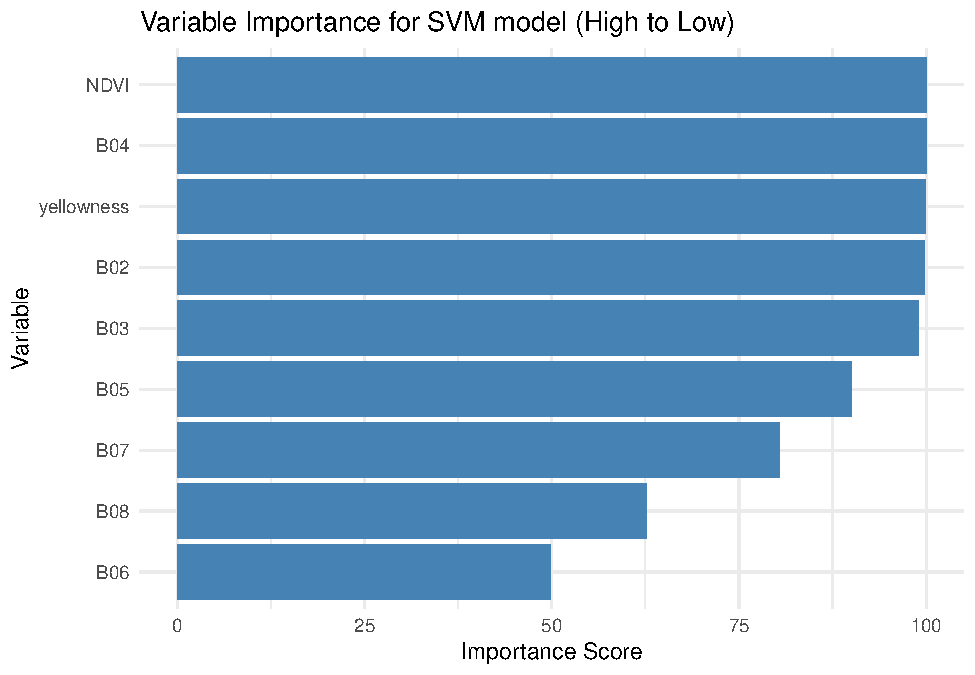
\includegraphics[keepaspectratio]{ML-based-modelling-for-spatial-and-spatiotemporal-data_files/figure-latex/svm_summary-1.pdf}}

The SVM model is trained, summary results and variable importance are
noted for the determining which predictor variable (sentinel bands) has
overall contributions to this classification.The variable importance
scores for each predictor variable is derived. The variable importance
plot shows which features contribute most to the classification task,
with the \texttt{NDVI}, \texttt{B04} \& \texttt{Yellowness} being among
the top 3 important predictors for the XGBoost model.

\textbf{Predicting the test data with confusion matrix and scoring
metrics:} To evaluate the performance of the SVM model on the test data
set, we can create a confusion matrix and calculate scoring metrics such
as accuracy, sensitivity, and specificity. The confusion matrix provides
insights into how well the model performs on the test data set.

\begin{Shaded}
\begin{Highlighting}[]
\CommentTok{\# Predict on the test dataset}
\NormalTok{predictions\_svm }\OtherTok{\textless{}{-}} \FunctionTok{predict}\NormalTok{(model\_svm, }
                           \AttributeTok{newdata =}\NormalTok{ testDat[, predictors])}
\NormalTok{probs\_svm }\OtherTok{\textless{}{-}} \FunctionTok{predict}\NormalTok{(model\_svm, }
                     \AttributeTok{newdata =}\NormalTok{ testDat[, predictors],}
                     \AttributeTok{probability =} \ConstantTok{TRUE}\NormalTok{)}

\CommentTok{\# Extract the levels from the training data response}
\NormalTok{true\_levels\_svm }\OtherTok{\textless{}{-}} \FunctionTok{levels}\NormalTok{(trainDat[[response]])}

\CommentTok{\# Convert both predicted and actual responses to factors with the same levels}
\NormalTok{predictions\_svm }\OtherTok{\textless{}{-}} \FunctionTok{factor}\NormalTok{(predictions\_svm, }
                          \AttributeTok{levels =}\NormalTok{ true\_levels\_svm)}
\NormalTok{actual\_svm }\OtherTok{\textless{}{-}} \FunctionTok{factor}\NormalTok{(testDat[[response]], }
                     \AttributeTok{levels =}\NormalTok{ true\_levels\_svm)}

\CommentTok{\# Construct the confusion matrix}
\NormalTok{confusion\_svm }\OtherTok{\textless{}{-}}\NormalTok{ caret}\SpecialCharTok{::}\FunctionTok{confusionMatrix}\NormalTok{(predictions\_svm, actual\_svm)}

\CommentTok{\# Plot confusion matrix}
\NormalTok{cm\_plot\_svm }\OtherTok{\textless{}{-}} \FunctionTok{ggplot}\NormalTok{(}\FunctionTok{as.data.frame}\NormalTok{(confusion\_svm}\SpecialCharTok{$}\NormalTok{table), }\FunctionTok{aes}\NormalTok{(}\AttributeTok{x =}\NormalTok{ Reference, }\AttributeTok{y =}\NormalTok{ Prediction)) }\SpecialCharTok{+}
  \FunctionTok{geom\_tile}\NormalTok{(}\FunctionTok{aes}\NormalTok{(}\AttributeTok{fill =}\NormalTok{ Freq), }\AttributeTok{color =} \StringTok{"white"}\NormalTok{) }\SpecialCharTok{+}
  \FunctionTok{scale\_fill\_gradient}\NormalTok{(}\AttributeTok{low =} \StringTok{"white"}\NormalTok{, }\AttributeTok{high =} \StringTok{"steelblue"}\NormalTok{) }\SpecialCharTok{+}
  \FunctionTok{geom\_text}\NormalTok{(}\FunctionTok{aes}\NormalTok{(}\AttributeTok{label =}\NormalTok{ Freq), }\AttributeTok{color =} \StringTok{"black"}\NormalTok{) }\SpecialCharTok{+}
  \FunctionTok{labs}\NormalTok{(}\AttributeTok{title =} \StringTok{"Confusion Matrix for Support Vector Machine Model"}\NormalTok{,}
       \AttributeTok{x =} \StringTok{"Reference Class"}\NormalTok{,}
       \AttributeTok{y =} \StringTok{"Predicted Class"}\NormalTok{) }\SpecialCharTok{+}
  \FunctionTok{theme\_minimal}\NormalTok{() }\SpecialCharTok{+}
  \FunctionTok{theme}\NormalTok{(}\AttributeTok{axis.text.x =} \FunctionTok{element\_text}\NormalTok{(}\AttributeTok{angle =} \DecValTok{45}\NormalTok{, }\AttributeTok{hjust =} \DecValTok{1}\NormalTok{))}

\CommentTok{\# Plot Confusion Matrix}
\NormalTok{cm\_plot\_svm}
\end{Highlighting}
\end{Shaded}

\pandocbounded{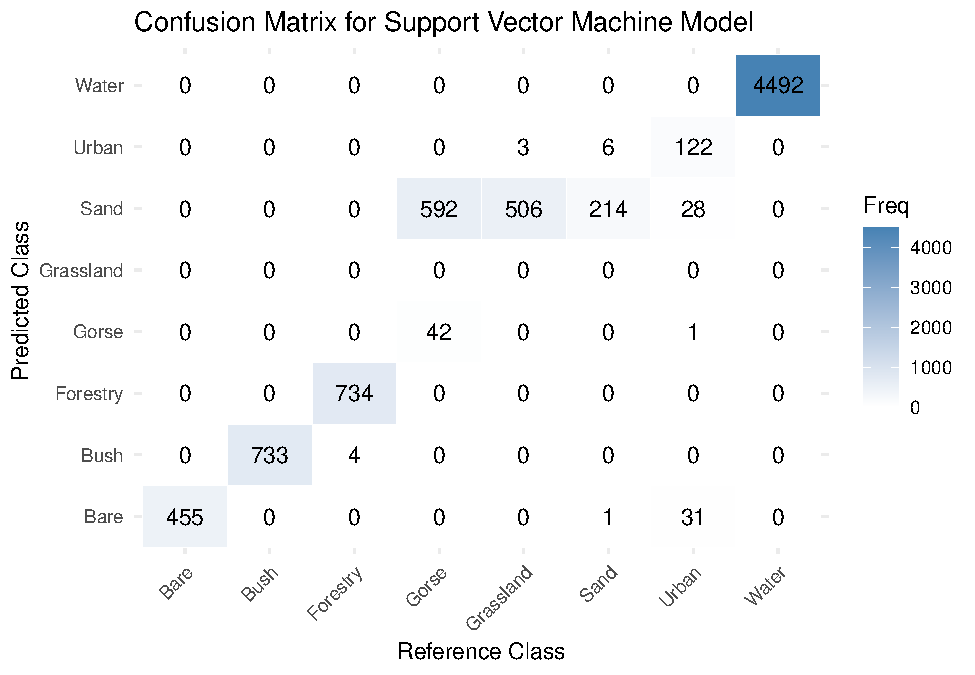
\includegraphics[keepaspectratio]{ML-based-modelling-for-spatial-and-spatiotemporal-data_files/figure-latex/svm_confusion_matrix-1.pdf}}

\begin{Shaded}
\begin{Highlighting}[]
\CommentTok{\# Print scoring metrics}
\FunctionTok{kable}\NormalTok{(confusion\_svm}\SpecialCharTok{$}\NormalTok{overall, }\AttributeTok{caption =} \StringTok{"Scoring Metrics for Support Vector Machine Model"}\NormalTok{) }\SpecialCharTok{\%\textgreater{}\%}
  \FunctionTok{kable\_styling}\NormalTok{(}\AttributeTok{full\_width =}\NormalTok{ F, }\AttributeTok{position =} \StringTok{"left"}\NormalTok{)}
\end{Highlighting}
\end{Shaded}

\begin{longtable}[l]{lr}
\caption{\label{tab:svm_confusion_matrix}Scoring Metrics for Support Vector Machine Model}\\
\toprule
 & x\\
\midrule
Accuracy & 0.8528378\\
Kappa & 0.7756107\\
AccuracyLower & 0.8448654\\
AccuracyUpper & 0.8605510\\
AccuracyNull & 0.5640382\\
\addlinespace
AccuracyPValue & 0.0000000\\
McnemarPValue & NaN\\
\bottomrule
\end{longtable}

\begin{Shaded}
\begin{Highlighting}[]
\CommentTok{\# Print sensitivity and specificity for each class}
\FunctionTok{kable}\NormalTok{(confusion\_svm}\SpecialCharTok{$}\NormalTok{byClass, }\AttributeTok{caption =} \StringTok{"Sensitivity and Specificity for Support Vector Machine Model"}\NormalTok{) }\SpecialCharTok{\%\textgreater{}\%}
  \FunctionTok{kable\_styling}\NormalTok{(}\AttributeTok{full\_width =}\NormalTok{ F, }\AttributeTok{position =} \StringTok{"left"}\NormalTok{)}
\end{Highlighting}
\end{Shaded}

\begin{longtable}[l]{lrrrrrrrrrrr}
\caption{\label{tab:svm_confusion_matrix}Sensitivity and Specificity for Support Vector Machine Model}\\
\toprule
 & Sensitivity & Specificity & Pos Pred Value & Neg Pred Value & Precision & Recall & F1 & Prevalence & Detection Rate & Detection Prevalence & Balanced Accuracy\\
\midrule
Class: Bare & 1.0000000 & 0.9957384 & 0.9342916 & 1.0000000 & 0.9342916 & 1.0000000 & 0.9660297 & 0.0571321 & 0.0571321 & 0.0611502 & 0.9978692\\
Class: Bush & 1.0000000 & 0.9994468 & 0.9945726 & 1.0000000 & 0.9945726 & 1.0000000 & 0.9972789 & 0.0920392 & 0.0920392 & 0.0925414 & 0.9997234\\
Class: Forestry & 0.9945799 & 1.0000000 & 1.0000000 & 0.9994467 & 1.0000000 & 0.9945799 & 0.9972826 & 0.0926670 & 0.0921647 & 0.0921647 & 0.9972900\\
Class: Gorse & 0.0662461 & 0.9998636 & 0.9767442 & 0.9252620 & 0.9767442 & 0.0662461 & 0.1240768 & 0.0796082 & 0.0052737 & 0.0053993 & 0.5330548\\
Class: Grassland & 0.0000000 & 1.0000000 & NaN & 0.9360874 & NA & 0.0000000 & NA & 0.0639126 & 0.0000000 & 0.0000000 & 0.5000000\\
\addlinespace
Class: Sand & 0.9683258 & 0.8545783 & 0.1597015 & 0.9989432 & 0.1597015 & 0.9683258 & 0.2741832 & 0.0277499 & 0.0268709 & 0.1682572 & 0.9114521\\
Class: Urban & 0.6703297 & 0.9988435 & 0.9312977 & 0.9923401 & 0.9312977 & 0.6703297 & 0.7795527 & 0.0228528 & 0.0153189 & 0.0164490 & 0.8345866\\
Class: Water & 1.0000000 & 1.0000000 & 1.0000000 & 1.0000000 & 1.0000000 & 1.0000000 & 1.0000000 & 0.5640382 & 0.5640382 & 0.5640382 & 1.0000000\\
\bottomrule
\end{longtable}

\textbf{Results} Confusion Matrix and scoring metrics provide insights
into the performance of the Support Vector Machine (SVM) model on the
test data set. The confusion matrix shows how many instances were highly
misclassified for each land cover class, while the scoring metrics
(accuracy, sensitivity, specificity) shows the model's poor performance.

The SVM model has not been trained successfully because the model
achieved poor performance having very low scores for the different
scoring matrix. The confusion matrix shows that the model has not
classified the defined land cover classes as there are lot of
misclassification. Hence the model does not fit this land cover
classification and will not be further used to compare the models and
assess the results and discussions of this project.

\section{5. Results \& Discussions}\label{results-discussions}

\subsection{Predicted maps}\label{predicted-maps}

Now the predicted model maps are visualized to check the land cover
classification and lay the training classes on the predicted models to
verify the classification visually.

\begin{Shaded}
\begin{Highlighting}[]
\CommentTok{\# Stacking Sentinel bands + indices}
\NormalTok{predictors\_stack }\OtherTok{\textless{}{-}} \FunctionTok{stack}\NormalTok{(sentinel}\SpecialCharTok{$}\NormalTok{B02, }
\NormalTok{                          sentinel}\SpecialCharTok{$}\NormalTok{B03, }
\NormalTok{                          sentinel}\SpecialCharTok{$}\NormalTok{B04, }
\NormalTok{                          sentinel}\SpecialCharTok{$}\NormalTok{B05,}
\NormalTok{                          sentinel}\SpecialCharTok{$}\NormalTok{B06, }
\NormalTok{                          sentinel}\SpecialCharTok{$}\NormalTok{B07, }
\NormalTok{                          sentinel}\SpecialCharTok{$}\NormalTok{B08,}
\NormalTok{                          sentinel}\SpecialCharTok{$}\NormalTok{NDVI, }
\NormalTok{                          sentinel}\SpecialCharTok{$}\NormalTok{yellowness)}

\CommentTok{\# Convert raster stack to dataframe (pixel wise)}
\NormalTok{pixels\_df }\OtherTok{\textless{}{-}} \FunctionTok{as.data.frame}\NormalTok{(predictors\_stack, }\AttributeTok{na.rm =} \ConstantTok{TRUE}\NormalTok{)}

\CommentTok{\# Predict for raster cells for each model}
\NormalTok{predictions\_rf }\OtherTok{\textless{}{-}} \FunctionTok{predict}\NormalTok{(model\_rf, }\AttributeTok{newdata =}\NormalTok{ pixels\_df, }\AttributeTok{type =} \StringTok{"raw"}\NormalTok{)}
\NormalTok{predictions\_xbg }\OtherTok{\textless{}{-}} \FunctionTok{predict}\NormalTok{(model\_xgb, }\AttributeTok{newdata =}\NormalTok{ pixels\_df, }\AttributeTok{type =} \StringTok{"raw"}\NormalTok{)}
\end{Highlighting}
\end{Shaded}

\begin{Shaded}
\begin{Highlighting}[]
\CommentTok{\# Create raster layers for each model prediction}
\NormalTok{raster\_rf  }\OtherTok{\textless{}{-}} \FunctionTok{setValues}\NormalTok{(}\FunctionTok{raster}\NormalTok{(predictors\_stack), predictions\_rf)}
\NormalTok{raster\_xgb }\OtherTok{\textless{}{-}} \FunctionTok{setValues}\NormalTok{(}\FunctionTok{raster}\NormalTok{(predictors\_stack), predictions\_xbg)}

\CommentTok{\# Define class names and palette}
\NormalTok{classes }\OtherTok{\textless{}{-}} \FunctionTok{c}\NormalTok{(}\StringTok{"Bare"}\NormalTok{, }\StringTok{"Bush"}\NormalTok{, }\StringTok{"Forestry"}\NormalTok{, }\StringTok{"Gorse"}\NormalTok{, }\StringTok{"Grassland"}\NormalTok{, }\StringTok{"Sand"}\NormalTok{, }\StringTok{"Urban"}\NormalTok{, }\StringTok{"Water"}\NormalTok{)}\CommentTok{\# Replace with your actual column name}
\NormalTok{class\_colors }\OtherTok{\textless{}{-}} \FunctionTok{c}\NormalTok{(}
  \StringTok{"Bare"}       \OtherTok{=} \StringTok{"\#a6643a"}\NormalTok{,   }\CommentTok{\# brown}
  \StringTok{"Bush"}       \OtherTok{=} \StringTok{"\#d01c8b"}\NormalTok{,   }\CommentTok{\# magenta}
  \StringTok{"Forestry"}   \OtherTok{=} \StringTok{"\#1b7837"}\NormalTok{,   }\CommentTok{\# dark green}
  \StringTok{"Gorse"}      \OtherTok{=} \StringTok{"\#ffff00"}\NormalTok{,   }\CommentTok{\# yellow}
  \StringTok{"Grassland"}  \OtherTok{=} \StringTok{"\#4dac26"}\NormalTok{,   }\CommentTok{\# light green}
  \StringTok{"Sand"}       \OtherTok{=} \StringTok{"\#f6e8c3"}\NormalTok{,   }\CommentTok{\# sand yellow}
  \StringTok{"Urban"}      \OtherTok{=} \StringTok{"\#878787"}\NormalTok{,   }\CommentTok{\# gray}
  \StringTok{"Water"}      \OtherTok{=} \StringTok{"\#4393c3"}    \CommentTok{\# blue}
\NormalTok{)}
\NormalTok{palette }\OtherTok{\textless{}{-}} \FunctionTok{unname}\NormalTok{(class\_colors[classes])}

\CommentTok{\# Convert to SpatRaster (terra) and assign class levels}
\NormalTok{raster\_rf  }\OtherTok{\textless{}{-}} \FunctionTok{rast}\NormalTok{(raster\_rf);  }\FunctionTok{levels}\NormalTok{(raster\_rf)  }\OtherTok{\textless{}{-}} \FunctionTok{data.frame}\NormalTok{(}\AttributeTok{value =} \DecValTok{1}\SpecialCharTok{:}\DecValTok{8}\NormalTok{, }\AttributeTok{class =}\NormalTok{ classes)}

\NormalTok{raster\_xgb }\OtherTok{\textless{}{-}} \FunctionTok{rast}\NormalTok{(raster\_xgb); }\FunctionTok{levels}\NormalTok{(raster\_xgb) }\OtherTok{\textless{}{-}} \FunctionTok{data.frame}\NormalTok{(}\AttributeTok{value =} \DecValTok{1}\SpecialCharTok{:}\DecValTok{8}\NormalTok{, }\AttributeTok{class =}\NormalTok{ classes)}

\FunctionTok{mapview}\NormalTok{(raster\_rf, }\AttributeTok{col.regions =}\NormalTok{ palette, }\AttributeTok{na.color =} \ConstantTok{NA}\NormalTok{) }\SpecialCharTok{+} 
  \FunctionTok{mapview}\NormalTok{(training, }\AttributeTok{zcol =} \StringTok{"Class"}\NormalTok{, }\AttributeTok{col.regions =} \StringTok{"black"}\NormalTok{, }\AttributeTok{alpha =} \FloatTok{0.5}\NormalTok{)}
\end{Highlighting}
\end{Shaded}

\begin{Shaded}
\begin{Highlighting}[]
\FunctionTok{mapview}\NormalTok{(raster\_xgb, }\AttributeTok{col.regions =}\NormalTok{ palette, }\AttributeTok{na.color =} \ConstantTok{NA}\NormalTok{) }\SpecialCharTok{+} 
  \FunctionTok{mapview}\NormalTok{(training, }\AttributeTok{zcol =} \StringTok{"Class"}\NormalTok{, }\AttributeTok{col.regions =} \StringTok{"black"}\NormalTok{, }\AttributeTok{alpha =} \FloatTok{0.5}\NormalTok{)}
\end{Highlighting}
\end{Shaded}

\textbf{Discussions:} The predicted thematic maps are overlayed with the
training land cover classes to visually validated the model performance.
Based on the maps, although there are slight misclassifications, both
the models shows utmost accurate classification as indicated by the
confusion matrix and scoring metrics. Out of the two,
\texttt{Random\ Forest} shows better performance in land cover
classification.

\subsection{Model Performance \& Uncertainly
Analysis}\label{model-performance-uncertainly-analysis}

Uncertainty analysis aims to quantify the reliability of predicted land
cover maps derived from remote sensing data.~It involves assessing and
managing errors and uncertainties associated with the classification
process, including those arising from data acquisition, processing, and
the classification algorithms themselves.~

\textbf{1. Confusion matrices \& Scoring metrics}

Comparing the Confusion matrices of the models, we can see how well each
model performed in classifying the land cover types. The confusion
matrices show the number of true positives, false positives, true
negatives, and false negatives for each class. This allows us to assess
the strengths and weaknesses of each model in terms of classification
accuracy.

\begin{Shaded}
\begin{Highlighting}[]
\CommentTok{\# Create a list of confusion matrices for each model}
\NormalTok{cm\_plot\_rf}
\end{Highlighting}
\end{Shaded}

\pandocbounded{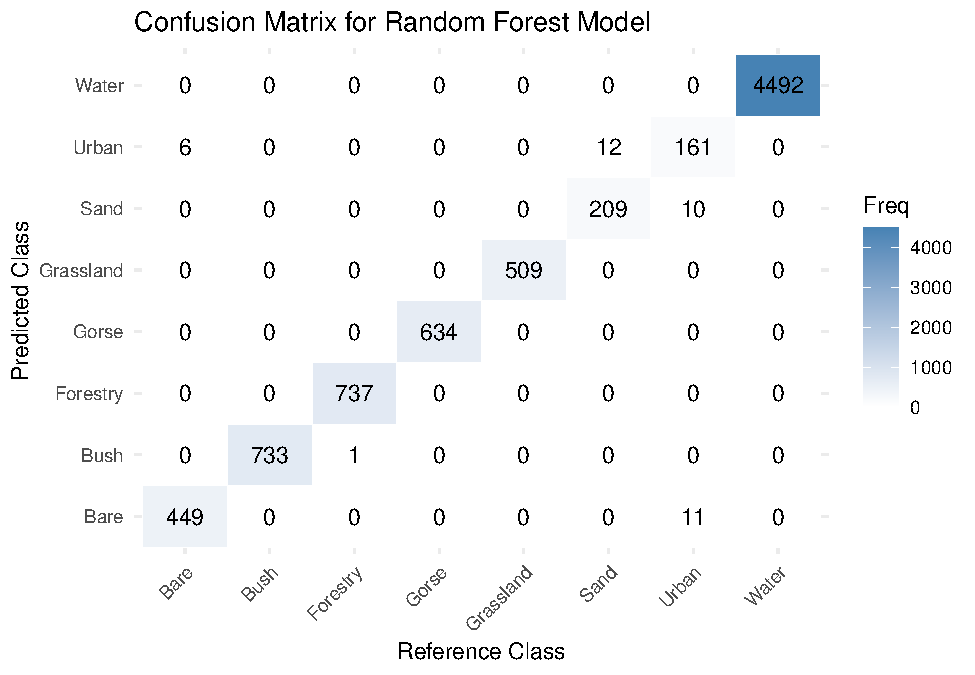
\includegraphics[keepaspectratio]{ML-based-modelling-for-spatial-and-spatiotemporal-data_files/figure-latex/confusion_matrices-1.pdf}}

\begin{Shaded}
\begin{Highlighting}[]
\NormalTok{cm\_plot\_xgb}
\end{Highlighting}
\end{Shaded}

\pandocbounded{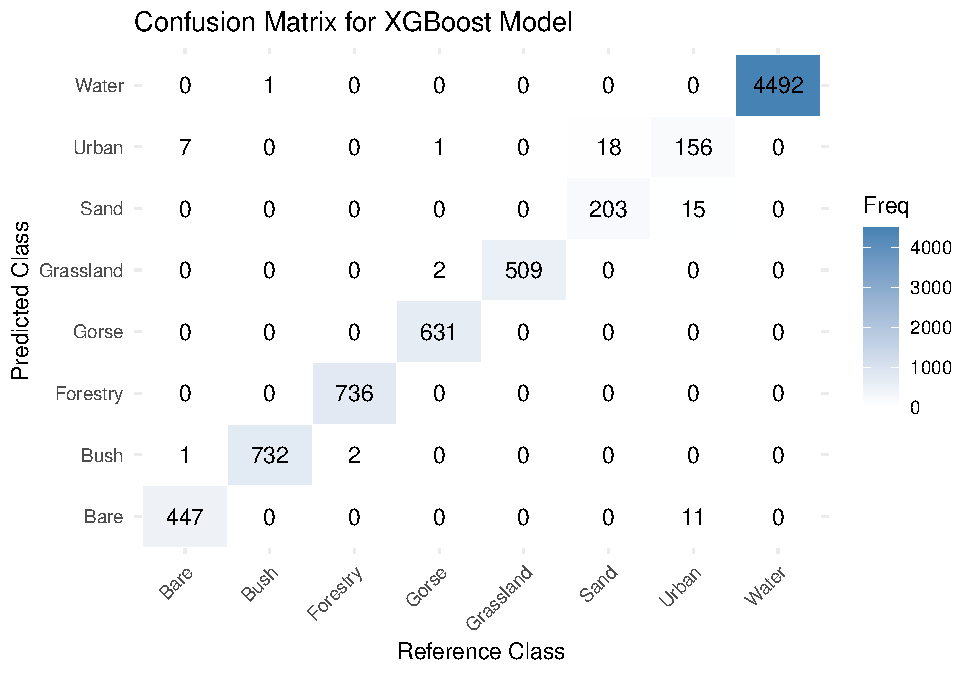
\includegraphics[keepaspectratio]{ML-based-modelling-for-spatial-and-spatiotemporal-data_files/figure-latex/confusion_matrices-2.pdf}}

Compare the scoring metrics (precision, f1score, recall, accuracy,
sensitivity, specificity) of the \texttt{RF} \& \texttt{XGBoost} models
to see which model performed best overall. The accuracy metric indicates
the overall correctness of the model, while sensitivity and specificity
provide insights into how well the model identifies each class.

\begin{Shaded}
\begin{Highlighting}[]
\CommentTok{\# Create a data frame to hold the scoring metrics for each model from the test dataset}
\NormalTok{scoring\_df }\OtherTok{\textless{}{-}} \FunctionTok{data.frame}\NormalTok{(}
  \AttributeTok{Metric =} \FunctionTok{c}\NormalTok{(}\StringTok{\textquotesingle{}Accuracy\textquotesingle{}}\NormalTok{, }\StringTok{\textquotesingle{}Kappa\textquotesingle{}}\NormalTok{, }\StringTok{\textquotesingle{}Precision\textquotesingle{}}\NormalTok{, }\StringTok{\textquotesingle{}Sensitivity\textquotesingle{}}\NormalTok{, }\StringTok{\textquotesingle{}Specificity\textquotesingle{}}\NormalTok{,}\StringTok{\textquotesingle{}F1\textquotesingle{}}\NormalTok{),}
  \AttributeTok{RandomForest =} \FunctionTok{c}\NormalTok{(confusion\_rf}\SpecialCharTok{$}\NormalTok{overall[}\StringTok{\textquotesingle{}Accuracy\textquotesingle{}}\NormalTok{],}
\NormalTok{                   confusion\_rf}\SpecialCharTok{$}\NormalTok{overall[}\StringTok{\textquotesingle{}Kappa\textquotesingle{}}\NormalTok{],}
                   \FunctionTok{mean}\NormalTok{(confusion\_rf}\SpecialCharTok{$}\NormalTok{byClass[,}\StringTok{"Precision"}\NormalTok{]),}
                   \FunctionTok{mean}\NormalTok{(confusion\_rf}\SpecialCharTok{$}\NormalTok{byClass[,}\StringTok{"Sensitivity"}\NormalTok{]),}
                   \FunctionTok{mean}\NormalTok{(confusion\_rf}\SpecialCharTok{$}\NormalTok{byClass[,}\StringTok{"Specificity"}\NormalTok{]),}
                   \FunctionTok{mean}\NormalTok{(confusion\_rf}\SpecialCharTok{$}\NormalTok{byClass[,}\StringTok{"F1"}\NormalTok{])),}
  \AttributeTok{XGBoost =} \FunctionTok{c}\NormalTok{(confusion\_xgb}\SpecialCharTok{$}\NormalTok{overall[}\StringTok{\textquotesingle{}Accuracy\textquotesingle{}}\NormalTok{],}
\NormalTok{              confusion\_xgb}\SpecialCharTok{$}\NormalTok{overall[}\StringTok{\textquotesingle{}Kappa\textquotesingle{}}\NormalTok{],}
              \FunctionTok{mean}\NormalTok{(confusion\_xgb}\SpecialCharTok{$}\NormalTok{byClass[,}\StringTok{"Precision"}\NormalTok{]),}
              \FunctionTok{mean}\NormalTok{(confusion\_xgb}\SpecialCharTok{$}\NormalTok{byClass[,}\StringTok{"Sensitivity"}\NormalTok{]),}
              \FunctionTok{mean}\NormalTok{(confusion\_xgb}\SpecialCharTok{$}\NormalTok{byClass[,}\StringTok{"Specificity"}\NormalTok{]),}
              \FunctionTok{mean}\NormalTok{(confusion\_rf}\SpecialCharTok{$}\NormalTok{byClass[,}\StringTok{"F1"}\NormalTok{])))}

\CommentTok{\# Print the scoring metrics data frame}
\FunctionTok{kable}\NormalTok{(scoring\_df, }\AttributeTok{caption =} \StringTok{"Scoring Metrics for Each Model"}\NormalTok{) }\SpecialCharTok{\%\textgreater{}\%}
  \FunctionTok{kable\_styling}\NormalTok{(}\AttributeTok{full\_width =}\NormalTok{ F, }\AttributeTok{position =} \StringTok{"left"}\NormalTok{)}
\end{Highlighting}
\end{Shaded}

\begin{longtable}[l]{lrr}
\caption{\label{tab:scoring_metrics}Scoring Metrics for Each Model}\\
\toprule
Metric & RandomForest & XGBoost\\
\midrule
Accuracy & 0.9949774 & 0.9927172\\
Kappa & 0.9922706 & 0.9887915\\
Precision & 0.9785630 & 0.9695125\\
Sensitivity & 0.9769719 & 0.9686633\\
Specificity & 0.9993490 & 0.9990357\\
\addlinespace
F1 & 0.9777535 & 0.9777535\\
\bottomrule
\end{longtable}

\begin{Shaded}
\begin{Highlighting}[]
\CommentTok{\# Convert to long format for plotting}
\NormalTok{scoring\_df\_long }\OtherTok{\textless{}{-}} \FunctionTok{melt}\NormalTok{(scoring\_df, }\AttributeTok{id.vars =} \StringTok{"Metric"}\NormalTok{,}
                        \AttributeTok{variable.name =} \StringTok{"Model"}\NormalTok{, }\AttributeTok{value.name =} \StringTok{"Score"}\NormalTok{)}
\CommentTok{\# Plot the scoring metrics for each model}
\FunctionTok{ggplot}\NormalTok{(scoring\_df\_long, }\FunctionTok{aes}\NormalTok{(}\AttributeTok{x =}\NormalTok{ Metric, }\AttributeTok{y =}\NormalTok{ Score, }\AttributeTok{fill =}\NormalTok{ Model)) }\SpecialCharTok{+}
  \FunctionTok{geom\_bar}\NormalTok{(}\AttributeTok{stat =} \StringTok{"identity"}\NormalTok{, }\AttributeTok{position =} \StringTok{"dodge"}\NormalTok{) }\SpecialCharTok{+}
  \FunctionTok{labs}\NormalTok{(}\AttributeTok{title =} \StringTok{"Scoring Metrics Comparison between the models"}\NormalTok{,}
       \AttributeTok{x =} \StringTok{"Metrix"}\NormalTok{, }\AttributeTok{y =} \StringTok{"Score"}\NormalTok{) }\SpecialCharTok{+}
  \FunctionTok{scale\_fill\_brewer}\NormalTok{(}\AttributeTok{palette =} \StringTok{"Set1"}\NormalTok{) }\SpecialCharTok{+}
  \FunctionTok{theme\_minimal}\NormalTok{() }\SpecialCharTok{+}
  \FunctionTok{theme}\NormalTok{(}\AttributeTok{axis.text.x =} \FunctionTok{element\_text}\NormalTok{(}\AttributeTok{angle =} \DecValTok{45}\NormalTok{, }\AttributeTok{hjust =} \DecValTok{1}\NormalTok{))}
\end{Highlighting}
\end{Shaded}

\pandocbounded{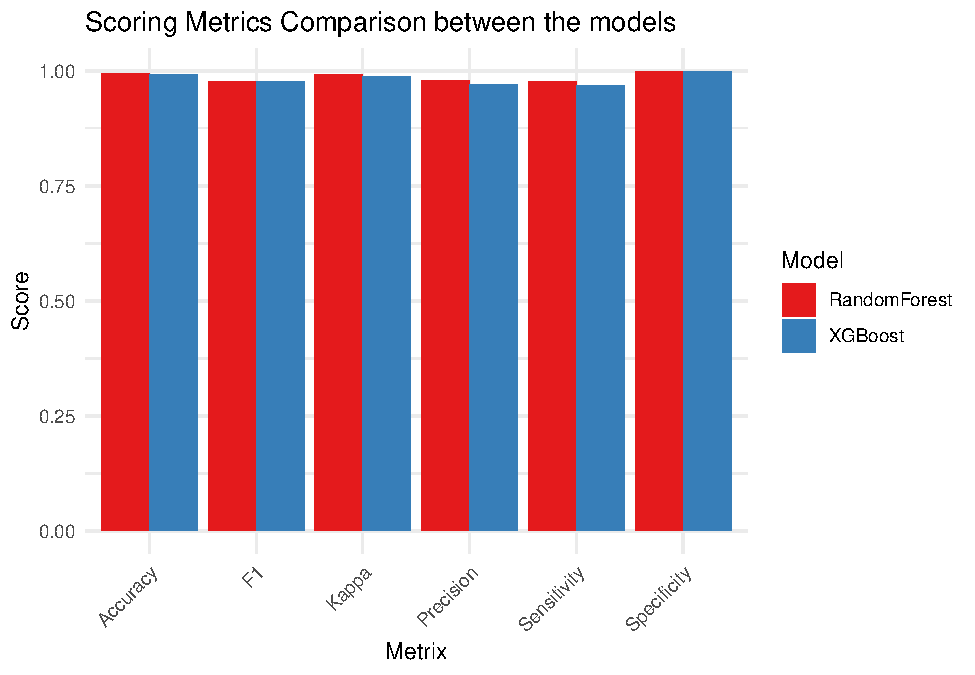
\includegraphics[keepaspectratio]{ML-based-modelling-for-spatial-and-spatiotemporal-data_files/figure-latex/scoring_metrics-1.pdf}}

\textbf{Discussion - Model Performance:} Confusion matrix from
\texttt{Random\ Forest} and \texttt{XGBoost} are shown here. As per the
results from the confusion matrix, the \texttt{Random\ Forest} Model
scores high true positives and very low false positives, when compared
with the \texttt{XGBoost} model. Furthermore, the scoring metrics
provide a comprehensive overview of the performance of each model. The
\texttt{Random\ Forest} model achieved the highest accuracy compared to
the \texttt{XGBoost}. The precision and sensitivity scores indicate that
Random Forest performed well in identifying the \textbf{gorse} class
than the \texttt{XGBoost}. The F1 score, which balances precision and
recall, also shows that \texttt{Random\ Forest} outperformed
\texttt{XGBoost}.

\textbf{2. Probability-based Entropy Maps (for uncertainty)} For this
uncertainity analysis, first predicting the class probabilities for the
models is required. With the predicted class probabilities, entropy per
pixel is calculated and then map these entropy values as a raster data.

\begin{Shaded}
\begin{Highlighting}[]
\CommentTok{\# Preparing the data}
\CommentTok{\# Convert the raster predictors to dataframe}
\NormalTok{pred\_data }\OtherTok{\textless{}{-}} \FunctionTok{as.data.frame}\NormalTok{(predictors\_stack, }\AttributeTok{na.rm =} \ConstantTok{TRUE}\NormalTok{)}
\NormalTok{valid\_idx }\OtherTok{\textless{}{-}} \FunctionTok{which}\NormalTok{(}\FunctionTok{complete.cases}\NormalTok{(pred\_data))}
\NormalTok{pred\_data\_valid }\OtherTok{\textless{}{-}}\NormalTok{ pred\_data[valid\_idx, ]}

\CommentTok{\# Predicting the model probabilities}
\NormalTok{prob\_rf }\OtherTok{\textless{}{-}} \FunctionTok{predict}\NormalTok{(model\_rf, pred\_data, }\AttributeTok{type=}\StringTok{\textquotesingle{}prob\textquotesingle{}}\NormalTok{)}
\NormalTok{prob\_xgb }\OtherTok{\textless{}{-}} \FunctionTok{predict}\NormalTok{(model\_xgb, pred\_data, }\AttributeTok{type=}\StringTok{\textquotesingle{}prob\textquotesingle{}}\NormalTok{)}

\CommentTok{\# Computing the entropy for the models}
\NormalTok{compute\_entropy }\OtherTok{\textless{}{-}} \ControlFlowTok{function}\NormalTok{ (p) \{}
\NormalTok{  epsilon }\OtherTok{\textless{}{-}} \FloatTok{1e{-}12} \CommentTok{\# Avoid log 0}
\NormalTok{  p }\OtherTok{\textless{}{-}} \FunctionTok{pmax}\NormalTok{(}\FunctionTok{pmin}\NormalTok{(p, }\DecValTok{1} \SpecialCharTok{{-}}\NormalTok{ epsilon), epsilon)  }\CommentTok{\# Clip values between epsilon and 1 {-} epsilon}
  \SpecialCharTok{{-}}\FunctionTok{rowSums}\NormalTok{(p }\SpecialCharTok{*} \FunctionTok{log2}\NormalTok{(p))}
\NormalTok{\}}

\CommentTok{\# Apply the model probabilitites to the entropy function}
\NormalTok{entropy\_rf }\OtherTok{\textless{}{-}} \FunctionTok{compute\_entropy}\NormalTok{(}\FunctionTok{as.matrix}\NormalTok{(prob\_rf))}
\NormalTok{entropy\_xgb }\OtherTok{\textless{}{-}} \FunctionTok{compute\_entropy}\NormalTok{(}\FunctionTok{as.matrix}\NormalTok{(prob\_xgb))}

\CommentTok{\# Setting up the plot}
\CommentTok{\# Create templates for the model}
\NormalTok{entropy\_raster\_rf }\OtherTok{\textless{}{-}}\NormalTok{ raster}\SpecialCharTok{::}\FunctionTok{raster}\NormalTok{(predictors\_stack)}
\NormalTok{entropy\_raster\_xgb }\OtherTok{\textless{}{-}}\NormalTok{ raster}\SpecialCharTok{::}\FunctionTok{raster}\NormalTok{(predictors\_stack)}

\CommentTok{\# Setting all values to NA}
\FunctionTok{values}\NormalTok{(entropy\_raster\_rf) }\OtherTok{\textless{}{-}} \ConstantTok{NA}
\FunctionTok{values}\NormalTok{(entropy\_raster\_xgb) }\OtherTok{\textless{}{-}} \ConstantTok{NA}

\CommentTok{\# Inserting the entropy values at valid locations}
\FunctionTok{values}\NormalTok{(entropy\_raster\_rf)[valid\_idx] }\OtherTok{\textless{}{-}}\NormalTok{ entropy\_rf}
\FunctionTok{values}\NormalTok{(entropy\_raster\_xgb)[valid\_idx] }\OtherTok{\textless{}{-}}\NormalTok{ entropy\_xgb}

\CommentTok{\# Convert raster to data frame for ggplot}
\CommentTok{\# Random Forest}
\NormalTok{df\_entropy\_rf }\OtherTok{\textless{}{-}} \FunctionTok{as.data.frame}\NormalTok{(entropy\_raster\_rf, }
                               \AttributeTok{xy =} \ConstantTok{TRUE}\NormalTok{, }\AttributeTok{na.rm =} \ConstantTok{TRUE}\NormalTok{)}
\FunctionTok{colnames}\NormalTok{(df\_entropy\_rf)[}\DecValTok{3}\NormalTok{] }\OtherTok{\textless{}{-}} \StringTok{"entropy"}
\CommentTok{\# XGBoost}
\NormalTok{df\_entropy\_xgb }\OtherTok{\textless{}{-}} \FunctionTok{as.data.frame}\NormalTok{(entropy\_raster\_xgb, }
                                \AttributeTok{xy =} \ConstantTok{TRUE}\NormalTok{, }\AttributeTok{na.rm =} \ConstantTok{TRUE}\NormalTok{)}
\FunctionTok{colnames}\NormalTok{(df\_entropy\_xgb)[}\DecValTok{3}\NormalTok{] }\OtherTok{\textless{}{-}} \StringTok{"entropy"}

\CommentTok{\# Create the ggplot for Random Forest entropy}
\NormalTok{p\_rf }\OtherTok{\textless{}{-}} \FunctionTok{ggplot}\NormalTok{(df\_entropy\_rf, }\FunctionTok{aes}\NormalTok{(}\AttributeTok{x =}\NormalTok{ x, }\AttributeTok{y =}\NormalTok{ y, }\AttributeTok{fill =}\NormalTok{ entropy)) }\SpecialCharTok{+}
  \FunctionTok{geom\_raster}\NormalTok{() }\SpecialCharTok{+}
  \FunctionTok{scale\_fill\_viridis}\NormalTok{(}\AttributeTok{option =} \StringTok{"viridis"}\NormalTok{) }\SpecialCharTok{+}
  \FunctionTok{coord\_equal}\NormalTok{() }\SpecialCharTok{+}
  \FunctionTok{labs}\NormalTok{(}\AttributeTok{title =} \StringTok{"Entropy {-} Random Forest"}\NormalTok{, }\AttributeTok{fill =} \StringTok{"Entropy"}\NormalTok{) }\SpecialCharTok{+}
  \FunctionTok{theme\_minimal}\NormalTok{()}

\CommentTok{\# Create the ggplot for XGBoost entropy}
\NormalTok{p\_xgb }\OtherTok{\textless{}{-}} \FunctionTok{ggplot}\NormalTok{(df\_entropy\_xgb, }\FunctionTok{aes}\NormalTok{(}\AttributeTok{x =}\NormalTok{ x, }\AttributeTok{y =}\NormalTok{ y, }\AttributeTok{fill =}\NormalTok{ entropy)) }\SpecialCharTok{+}
  \FunctionTok{geom\_raster}\NormalTok{() }\SpecialCharTok{+}
  \FunctionTok{scale\_fill\_viridis}\NormalTok{(}\AttributeTok{option =} \StringTok{"viridis"}\NormalTok{) }\SpecialCharTok{+}
  \FunctionTok{coord\_equal}\NormalTok{() }\SpecialCharTok{+}
  \FunctionTok{labs}\NormalTok{(}\AttributeTok{title =} \StringTok{"Entropy {-} XGBoost"}\NormalTok{, }\AttributeTok{fill =} \StringTok{"Entropy"}\NormalTok{) }\SpecialCharTok{+}
  \FunctionTok{theme\_minimal}\NormalTok{()         }

\CommentTok{\# Plot the entropy maps}
\FunctionTok{par}\NormalTok{(}\AttributeTok{mfrow=}\FunctionTok{c}\NormalTok{(}\DecValTok{1}\NormalTok{,}\DecValTok{2}\NormalTok{))}
\NormalTok{p\_rf}
\end{Highlighting}
\end{Shaded}

\pandocbounded{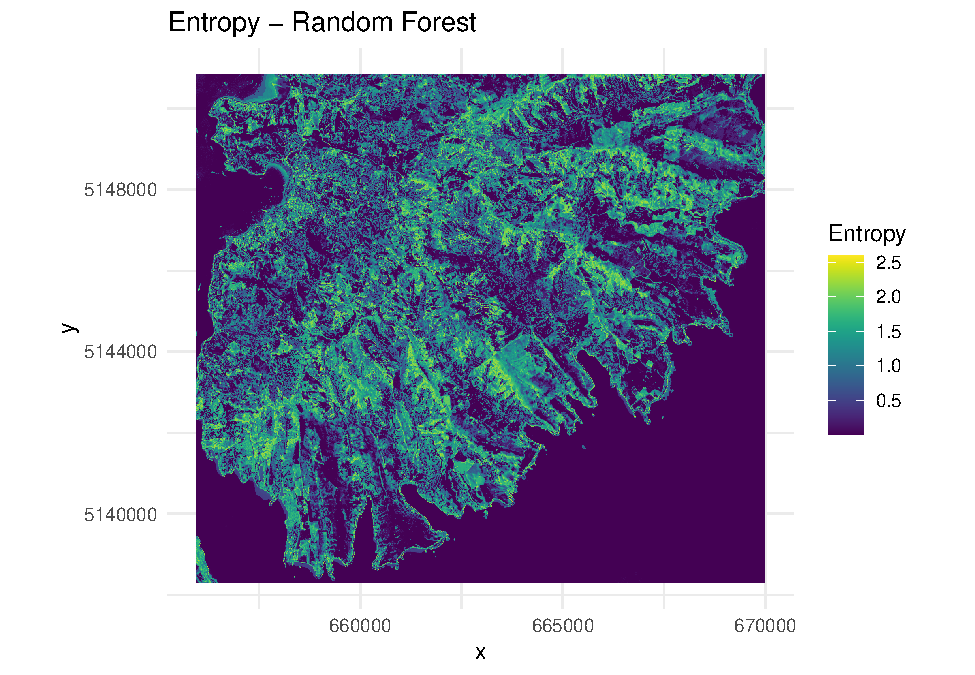
\includegraphics[keepaspectratio]{ML-based-modelling-for-spatial-and-spatiotemporal-data_files/figure-latex/entropy map-1.pdf}}

\begin{Shaded}
\begin{Highlighting}[]
\NormalTok{p\_xgb}
\end{Highlighting}
\end{Shaded}

\pandocbounded{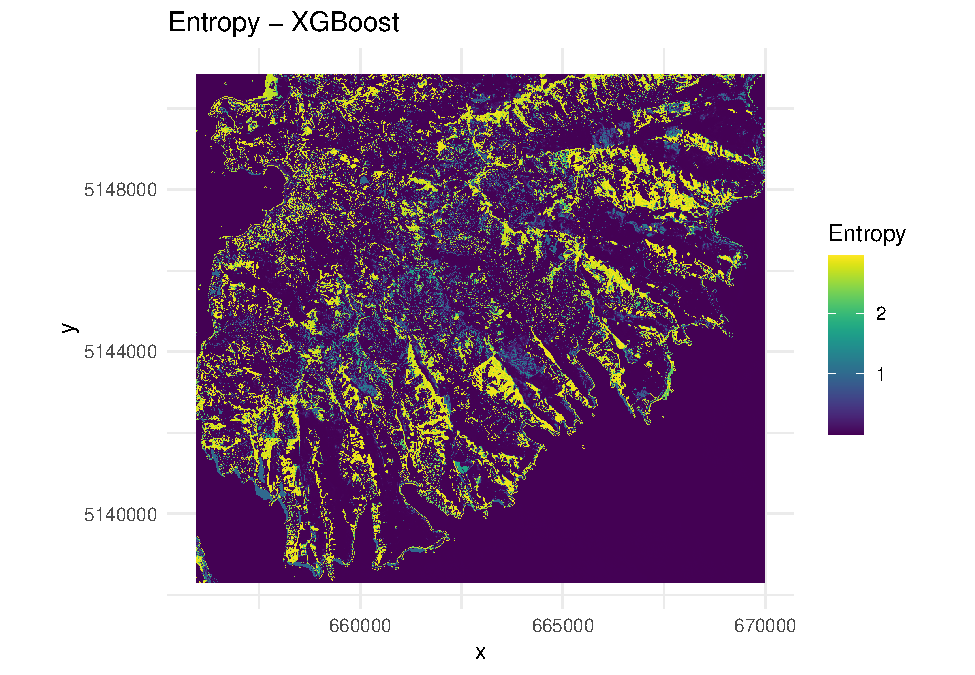
\includegraphics[keepaspectratio]{ML-based-modelling-for-spatial-and-spatiotemporal-data_files/figure-latex/entropy map-2.pdf}}

\begin{Shaded}
\begin{Highlighting}[]
\FunctionTok{par}\NormalTok{(}\AttributeTok{mfrow=}\FunctionTok{c}\NormalTok{(}\DecValTok{1}\NormalTok{,}\DecValTok{1}\NormalTok{))                               }
\end{Highlighting}
\end{Shaded}

\textbf{Discussion} These entropy maps shows the uncertainity in the
predictions in the model. More yellow the higher entropy and more purple
the lower entropy. Low entropy signifies the confidence in predictions
where high entropy shows the uncertaininty and might be similar
probabilities to multiple class. In these maps, RF entropy maps shows
more gradual transitions and less extreme entropy which means that the
model could be robust to noise and less flexible. On the contrary,
XGBoost shows sharper contrasts and more high entropy areas particularty
at the class boundaries. This could mean the model classification is
sensitive to the class boundaries and also could be the problem of
overfitting.

\textbf{3. DALEX Uncertainity Analysis} To gain insights into the
uncertainty of the model predictions, we can use the DALEX (Descriptive
mAchine Learning EXplanations) package designed to help understand and
explain complex machine learning models. DALEX allows to explore the
model performance and diagnostics for each model. This allows us to
analyze the model's predictions and understand how different features
contribute to the uncertainty in the predictions.

\begin{Shaded}
\begin{Highlighting}[]
\CommentTok{\# DALEX {-} Prediction Diagnostics}
\CommentTok{\# Define a safe predict function}
\NormalTok{predict\_class }\OtherTok{\textless{}{-}} \ControlFlowTok{function}\NormalTok{(m, d) }\FunctionTok{predict}\NormalTok{(m, d, }\AttributeTok{type =} \StringTok{"raw"}\NormalTok{)}

\CommentTok{\# Create explainers for each model using DALEX}
\NormalTok{explainer\_rf }\OtherTok{\textless{}{-}}\NormalTok{ DALEX}\SpecialCharTok{::}\FunctionTok{explain}\NormalTok{(model\_rf, }
                               \AttributeTok{data =}\NormalTok{ testDat[, predictors], }
                               \AttributeTok{y =}\NormalTok{ testDat}\SpecialCharTok{$}\NormalTok{Class, }
                               \AttributeTok{label =} \StringTok{"Random Forest"}\NormalTok{)}
\end{Highlighting}
\end{Shaded}

\begin{verbatim}
## Preparation of a new explainer is initiated
##   -> model label       :  Random Forest 
##   -> data              :  7964  rows  9  cols 
##   -> target variable   :  7964  values 
##   -> predict function  :  yhat.train  will be used (  default  )
##   -> predicted values  :  No value for predict function target column. (  default  )
##   -> model_info        :  package caret , ver. 7.0.1 , task multiclass (  default  ) 
##   -> predicted values  :  predict function returns multiple columns:  8  (  default  ) 
##   -> residual function :  difference between 1 and probability of true class (  default  )
##   -> residuals         :  numerical, min =  0 , mean =  0.01093245 , max =  0.996  
##   A new explainer has been created!
\end{verbatim}

\begin{Shaded}
\begin{Highlighting}[]
\NormalTok{explainer\_xgb }\OtherTok{\textless{}{-}}\NormalTok{ DALEX}\SpecialCharTok{::}\FunctionTok{explain}\NormalTok{(model\_xgb, }
                                \AttributeTok{data =}\NormalTok{ testDat[, predictors], }
                                \AttributeTok{y =}\NormalTok{ testDat}\SpecialCharTok{$}\NormalTok{Class, }
                                \AttributeTok{label =} \StringTok{"XGBoost"}\NormalTok{)}
\end{Highlighting}
\end{Shaded}

\begin{verbatim}
## Preparation of a new explainer is initiated
##   -> model label       :  XGBoost 
##   -> data              :  7964  rows  9  cols 
##   -> target variable   :  7964  values 
##   -> predict function  :  yhat.train  will be used (  default  )
##   -> predicted values  :  No value for predict function target column. (  default  )
##   -> model_info        :  package caret , ver. 7.0.1 , task multiclass (  default  ) 
##   -> predicted values  :  predict function returns multiple columns:  8  (  default  ) 
##   -> residual function :  difference between 1 and probability of true class (  default  )
##   -> residuals         :  numerical, min =  1.502037e-05 , mean =  0.007651202 , max =  0.9999674  
##   A new explainer has been created!
\end{verbatim}

\begin{Shaded}
\begin{Highlighting}[]
\CommentTok{\# Take 5 random observations from the test set}
\FunctionTok{set.seed}\NormalTok{(}\DecValTok{123}\NormalTok{)}
\NormalTok{new\_obs }\OtherTok{\textless{}{-}}\NormalTok{ testDat[}\DecValTok{1}\NormalTok{, predictors]}
\CommentTok{\# Compute diagnostics for each model}
\NormalTok{diag\_rf }\OtherTok{\textless{}{-}} \FunctionTok{predict\_diagnostics}\NormalTok{(explainer\_rf, }
                               \AttributeTok{new\_observation =}\NormalTok{  new\_obs, }\AttributeTok{N=}\ConstantTok{NULL}\NormalTok{)}
\NormalTok{diag\_xgb }\OtherTok{\textless{}{-}} \FunctionTok{predict\_diagnostics}\NormalTok{(explainer\_xgb, }
                                \AttributeTok{new\_observation =}\NormalTok{ new\_obs, }\AttributeTok{N=}\ConstantTok{NULL}\NormalTok{)}

\CommentTok{\# Plotting uncertainty histograms}
\NormalTok{hist\_rf }\OtherTok{\textless{}{-}} \FunctionTok{rbind}\NormalTok{(diag\_rf}\SpecialCharTok{$}\NormalTok{histogram\_neighbors, diag\_rf}\SpecialCharTok{$}\NormalTok{histogram\_all)}
\NormalTok{hist\_rf}\SpecialCharTok{$}\NormalTok{model }\OtherTok{\textless{}{-}} \StringTok{"Random Forest"}

\NormalTok{hist\_xgb }\OtherTok{\textless{}{-}} \FunctionTok{rbind}\NormalTok{(diag\_xgb}\SpecialCharTok{$}\NormalTok{histogram\_neighbors, diag\_xgb}\SpecialCharTok{$}\NormalTok{histogram\_all)}
\NormalTok{hist\_xgb}\SpecialCharTok{$}\NormalTok{model }\OtherTok{\textless{}{-}} \StringTok{"XGBoost"}

\CommentTok{\# Combine all}
\NormalTok{combined\_hist }\OtherTok{\textless{}{-}} \FunctionTok{rbind}\NormalTok{(hist\_rf, hist\_xgb)}

\CommentTok{\# Plotting the histogram }
\FunctionTok{ggplot}\NormalTok{(combined\_hist, }\FunctionTok{aes}\NormalTok{(}\AttributeTok{x =}\NormalTok{ Var1, }\AttributeTok{y =}\NormalTok{ Freq, }\AttributeTok{fill =}\NormalTok{ direction)) }\SpecialCharTok{+}
  \FunctionTok{geom\_bar}\NormalTok{(}\AttributeTok{stat =} \StringTok{"identity"}\NormalTok{, }\AttributeTok{position =} \StringTok{"dodge"}\NormalTok{) }\SpecialCharTok{+}
  \FunctionTok{facet\_wrap}\NormalTok{(}\SpecialCharTok{\textasciitilde{}}\NormalTok{model, }\AttributeTok{scales =} \StringTok{"free\_y"}\NormalTok{) }\SpecialCharTok{+}
  \FunctionTok{scale\_fill\_manual}\NormalTok{(}\AttributeTok{values =} \FunctionTok{c}\NormalTok{(}\StringTok{"neighbors"} \OtherTok{=} \StringTok{"steelblue"}\NormalTok{, }\StringTok{"all"} \OtherTok{=} \StringTok{"tomato"}\NormalTok{)) }\SpecialCharTok{+}
  \FunctionTok{theme\_minimal}\NormalTok{() }\SpecialCharTok{+}
  \FunctionTok{labs}\NormalTok{(}\AttributeTok{title =} \StringTok{"Similarity to Training Data"}\NormalTok{,}
       \AttributeTok{x =} \StringTok{"Distance Bin"}\NormalTok{,}
       \AttributeTok{y =} \StringTok{"Frequency"}\NormalTok{,}
       \AttributeTok{fill =} \StringTok{"Compared To"}\NormalTok{) }\SpecialCharTok{+}
  \FunctionTok{theme}\NormalTok{(}\AttributeTok{axis.text.x =} \FunctionTok{element\_text}\NormalTok{(}\AttributeTok{angle =} \DecValTok{45}\NormalTok{, }\AttributeTok{hjust =} \DecValTok{1}\NormalTok{, , }\AttributeTok{size =} \DecValTok{5}\NormalTok{))}
\end{Highlighting}
\end{Shaded}

\pandocbounded{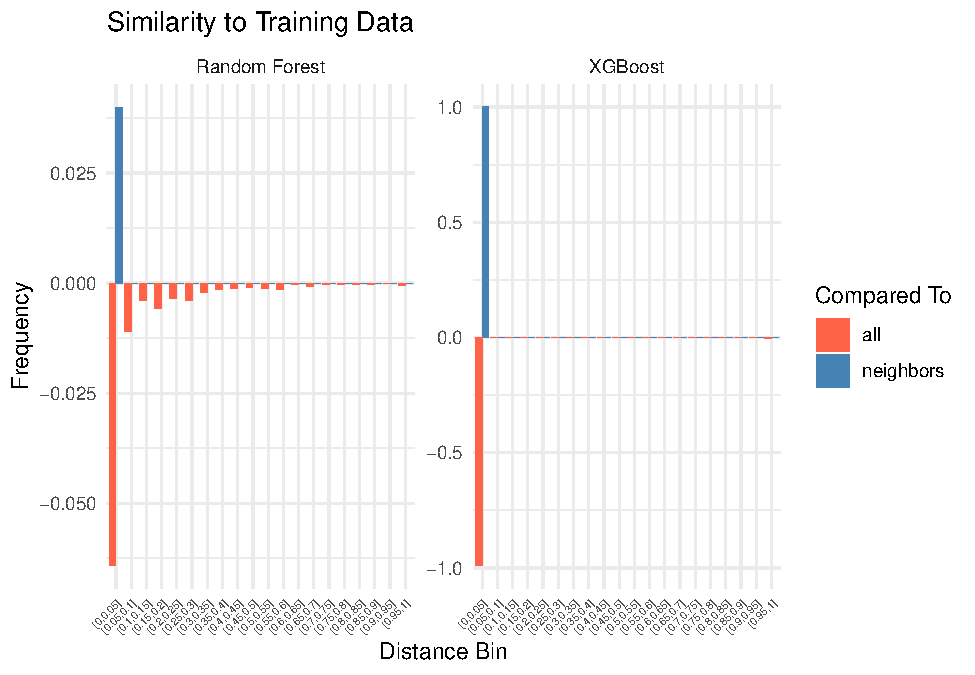
\includegraphics[keepaspectratio]{ML-based-modelling-for-spatial-and-spatiotemporal-data_files/figure-latex/uncertainty_analysis-1.pdf}}

\textbf{Discussion:} Both the models show a sharp spike at very low bin
distance bins which means that the test dataset is highly similar to the
training dataset, particularly in the XGBoost. This suggests that both
models use very similar training data to make predictions. In the RF
model, the model red bar are all negative, which shows that the test
data as a whole is less similar to the entire training data
distribution. This suggests that the RF model has some overfitting and
learned well from local structures. From both the plots, RF has more
spread across the bin whereas the XGBoost has a sharp spike at the
lowest bin. This shows that the XGBoost heavily relies on few highly
similar instances, whereas RF has spreads its attention.

\section{6. Conclusion}\label{conclusion}

The project aim is to predict the invasive species \textbf{gorse
(\emph{Ulex europaeus})} on the Banks Peninsula in New Zealand. Based
this project goal, using the Sentinel satellite images and plotted land
cover class data shapes of the study area, three machine learning models
(\texttt{Random\ Forest\ (RF)}, \texttt{XGBoost} \&
\texttt{Support\ Vector\ Machine\ (SVM)} are selected and trained with
similar training control methods (Cross validation method and k-fold at
10). Out of the three models, \texttt{RF} and \texttt{XGBoost} model
performs very well and \texttt{SVM} model is not upto par in classifying
the land cover class using the satellite images.

Based on various analysis such as confusion matrix, scoring metrics,
predictive \& entropy maps, and uncertainy diagonostics, \texttt{RF}
model has low uncertainty and predicts the land cover classes with the
highest accuracy of 99.33\%, when compared to the \texttt{XGBoost}. In
conclusion, \texttt{Random\ Forest} Model outperforms \texttt{XGBoost}
in predicting the invasive species \textbf{gorse (\emph{Ulex
europaeus})}, using Sentinel satellite data, on the Banks Peninsula of
New Zealand.

\end{document}
